% Supplementary material for the thesis.
%
% Five appendices are bound here rather than in the thesis body, because none
% of them is read sequentially and the thesis's own Appendix A already points
% a reader to this file by name for each one: Appendix B is the complete
% correction record, Appendix C is the register of reported quantities,
% Appendix D is the claim-and-evidence trace, Appendix E is the survey coding
% table (75 papers), and Appendix F is the full quantitative treatment of the
% selection-channel anomaly. Appendices B, C and D are machine-generated, by
% accord/stats/make_appendices.py (B and C) and accord/stats/trace_claims.py
% (D), from the project records, so none of the three can drift from the
% source it describes. FORMAT.md records no page limit for the thesis, so no
% page-limit reason is given for binding these here; the reason is only that
% none of the five is read sequentially.
%
% Nothing is abbreviated. Every table is reproduced complete.
%
% Build:  pdflatex main_supplement && pdflatex main_supplement

\documentclass[12pt]{report}

\usepackage[left=1.5in,right=1in,top=1in,bottom=1in,includefoot]{geometry}
\usepackage{mathptmx}
\usepackage{courier}
\usepackage[T1]{fontenc}
% t1pcr.fd defines \hyphenchar\font\m@ne, so @ has to be a letter here,
% exactly as in main_msu.tex. Without \makeatletter this throws on every
% typewriter glyph the tables use.
%
% Copied verbatim from main_msu.tex (its \DeclareFontShape block). Without
% these, NFSS falls through to its own automatic series/shape substitution
% search for every series/shape combination \touchttfonts primes for
% \texttt hyphenation that t1pcr.fd does not itself define, which is what
% raised 23 "Some font shapes were not available" warnings in this
% document's log even though none of these shapes render visible text here.
\makeatletter
\input{t1pcr.fd}
\DeclareFontShape{T1}{pcr}{sb}{n}{<->ssub * pcr/b/n}{}
\DeclareFontShape{T1}{pcr}{sb}{it}{<->ssub * pcr/b/it}{}
\DeclareFontShape{T1}{pcr}{sb}{sl}{<->ssub * pcr/b/sl}{}
\DeclareFontShape{T1}{pcr}{sb}{sc}{<->ssub * pcr/b/sc}{}
\DeclareFontShape{T1}{pcr}{c}{n}{<->ssub * pcr/m/n}{}
\DeclareFontShape{T1}{pcr}{c}{it}{<->ssub * pcr/m/it}{}
\DeclareFontShape{T1}{pcr}{c}{sl}{<->ssub * pcr/m/sl}{}
\DeclareFontShape{T1}{pcr}{c}{sc}{<->ssub * pcr/m/sc}{}
\DeclareFontShape{T1}{pcr}{l}{n}{<->ssub * pcr/m/n}{}
\DeclareFontShape{T1}{pcr}{l}{it}{<->ssub * pcr/m/it}{}
\DeclareFontShape{T1}{pcr}{l}{sl}{<->ssub * pcr/m/sl}{}
\DeclareFontShape{T1}{pcr}{l}{sc}{<->ssub * pcr/m/sc}{}
\DeclareFontShape{T1}{pcr}{m}{ui}{<->ssub * pcr/m/it}{}
\DeclareFontShape{T1}{pcr}{bx}{ui}{<->ssub * pcr/bx/it}{}
\DeclareFontShape{T1}{pcr}{m}{In}{<->ssub * pcr/m/n}{}
\DeclareFontShape{T1}{pcr}{m}{scsl}{<->ssub * pcr/m/sc}{}
\DeclareFontShape{T1}{pcr}{b}{scsl}{<->ssub * pcr/b/sc}{}
\DeclareFontShape{T1}{pcr}{bx}{scsl}{<->ssub * pcr/bx/sc}{}
\DeclareFontShape{T1}{pcr}{bc}{sc}{<->ssub * pcr/b/sc}{}
\DeclareFontShape{T1}{pcr}{c}{scsl}{<->ssub * pcr/m/sc}{}
\DeclareFontShape{T1}{pcr}{sbx}{n}{<->ssub * pcr/b/n}{}
\DeclareFontShape{T1}{pcr}{sbx}{it}{<->ssub * pcr/b/it}{}
\DeclareFontShape{T1}{pcr}{sbx}{sl}{<->ssub * pcr/b/sl}{}
\DeclareFontShape{T1}{pcr}{sbx}{sc}{<->ssub * pcr/b/sc}{}
\DeclareFontShape{T1}{pcr}{lc}{n}{<->ssub * pcr/m/n}{}
\DeclareFontShape{T1}{pcr}{lc}{it}{<->ssub * pcr/m/it}{}
\DeclareFontShape{T1}{pcr}{lc}{sl}{<->ssub * pcr/m/sl}{}
\DeclareFontShape{T1}{pcr}{lc}{sc}{<->ssub * pcr/m/sc}{}
\DeclareFontShape{T1}{pcr}{lc}{scsl}{<->ssub * pcr/m/sc}{}
\DeclareFontShape{T1}{pcr}{sbc}{sc}{<->ssub * pcr/b/sc}{}
\DeclareFontShape{T1}{pcr}{sbx}{scsl}{<->ssub * pcr/b/sc}{}
\DeclareFontShape{T1}{pcr}{sbc}{scsl}{<->ssub * pcr/b/sc}{}
\DeclareFontShape{T1}{pcr}{sbc}{n}{<->ssub * pcr/b/n}{}
\DeclareFontShape{T1}{pcr}{sbc}{it}{<->ssub * pcr/b/it}{}
\DeclareFontShape{T1}{pcr}{sbc}{sl}{<->ssub * pcr/b/sl}{}
\DeclareFontShape{T1}{pcr}{sbc}{scit}{<->ssub * pcr/b/sc}{}
\makeatother
\usepackage[utf8]{inputenc}
% graphicx was absent, so every \includegraphics in the appendices raised
% Undefined control sequence and the supplement built to a broken PDF that
% nothing checked: the verification harness reads main_msu.pdf only, and
% build.sh did not build this document at all.
\usepackage{graphicx}
\usepackage{float}
\usepackage{longtable}
\usepackage{booktabs}
\usepackage{setspace}
% caption was absent, so \captionsetup below had nothing to configure and
% every caption in this document fell back to LaTeX's plain default style,
% ignoring the labelling and positioning main_msu.tex sets for the thesis.
\usepackage{caption}
\usepackage{titlesec}
\usepackage[htt]{hyphenat}
\usepackage[hidelinks]{hyperref}

\renewcommand{\familydefault}{\rmdefault}
\doublespacing
\setlength{\parindent}{0.5in}
% Copied from main_msu.tex: MSU's 0.5in first-line indent, no paragraph skip,
% and the widow/orphan controls it sets alongside them. This document had
% none of the three, so a paragraph break here read differently from the
% same paragraph convention in the thesis it supplements.
\setlength{\parskip}{0pt}
\frenchspacing
\clubpenalty=10000
\widowpenalty=10000
\displaywidowpenalty=10000

% Copied verbatim from main_msu.tex. The appendix files are shared between the
% two documents, so a macro they use has to mean the same thing in both.
\newcommand{\apanote}[1]{%
  \par\vspace{0.25\baselineskip}%
  \begingroup\raggedright\noindent\textit{Note.} #1\par\endgroup}

% Figures, tables and equations number consecutively within this document,
% not per appendix. (Same fix as main_msu.tex lines 128-134: without it the
% one figure in Appendix F printed as "Figure F.1" instead of "Figure 1".)
\makeatletter
\@removefromreset{figure}{chapter}
\@removefromreset{table}{chapter}
\@removefromreset{equation}{chapter}
\makeatother
\renewcommand{\thefigure}{\arabic{figure}}
\renewcommand{\thetable}{\arabic{table}}
\renewcommand{\theequation}{\arabic{equation}}

\setcounter{secnumdepth}{2}

\titleformat{\chapter}[block]
  {\normalfont\centering\bfseries\normalsize}
  {Appendix \thechapter:}{0.5em}{}
\titlespacing*{\chapter}{0pt}{0pt}{0.3in}

% Sections were printing their number ("B.1") on its own line above the
% heading text, because titlesec was loaded (for the chapter format above)
% but never given a \titleformat for \section or \subsection, so both fell
% back to LaTeX's default numbered heading. Copied from main_msu.tex, which
% suppresses the printed number the same way while secnumdepth above still
% lets it appear in a table of contents if one is ever added to this file.
\titleformat{\section}{\normalfont\bfseries\normalsize}{}{0pt}{}
\titlespacing*{\section}{0pt}{\baselineskip}{0.4\baselineskip}

\titleformat{\subsection}{\normalfont\bfseries\itshape\normalsize}{}{0pt}{}
\titlespacing*{\subsection}{0pt}{0.75\baselineskip}{0.35\baselineskip}

% Matches main_msu.tex's \captionsetup exactly. This document had no \captionsetup at all, so every caption used LaTeX's
% plain, unlabelled default, and Appendix F's figure caption happened to land
% below by coincidence of source order rather than by any rule. The convention
% here matches the main document: FORMAT.md section 5, bold label on its own
% line, italic text beneath, above both figures and tables. The main document
% followed the departmental example instead until the citation style was moved
% to APA 7 on section 8's authority, at which point holding section 5 apart from
% it stopped being defensible.
\captionsetup[figure]{labelsep=newline,labelfont=bf,textfont=it,
  font={normalsize,stretch=1},justification=justified,singlelinecheck=false,
  position=top,skip=0.6\baselineskip}
\captionsetup[table]{labelsep=newline,labelfont=bf,textfont=it,
  font={normalsize,stretch=1},justification=justified,singlelinecheck=false,
  position=top,skip=0.6\baselineskip}

\begin{document}

\pagenumbering{roman}
\thispagestyle{empty}
\vspace*{1.4in}
\begin{center}
  {\normalsize\bfseries SUPPLEMENTARY MATERIAL\par}
  \vspace{0.3in}
  {\normalsize Why a Cross-Note Medication Contradiction Detection Pipeline Fails:\\
   A Controlled Failure Analysis\par}
  \vspace{0.3in}
  Ricky Gole\par
  \vspace{0.6in}
  MORGAN STATE UNIVERSITY\par
\end{center}

\vspace{0.8in}
% This paragraph named every appendix one letter too low: \setcounter{chapter}{1}
% below shifts the first appendix bound here to B, not A, and the letters after
% it shift the same way, but the prose describing them was written before that
% shift and was never updated to match what actually prints. It also covered
% only three of the five appendices this file binds. Rewritten against the
% printed headings, verified with pdftotext against the built PDF.
\noindent This file binds five appendices. Appendix B reproduces every
correction issued during the work, not only the ten that the thesis's own
Appendix A prints because they changed a number the thesis still reports.
Appendix C is the register of reported quantities, and Appendix D traces
every quantity printed in the thesis to the file it was read from; both are
generated by \texttt{accord/stats/make\_appendices.py} and
\texttt{accord/stats/trace\_claims.py} from the project records, so neither
can drift from the source it describes. Appendix E reproduces the coding of
all 75 surveyed papers behind the prevalence measurement in the thesis.
Appendix F is the full quantitative treatment of the selection-channel
anomaly that the thesis's discussion chapter reports only in summary. In
Appendices C and D, the redaction [LOCAL] marks a file path that exists only
on the author's own machine and [DRIVE] marks a path on a shared drive; both
are path redactions, not unfilled placeholders.

\clearpage
\pagenumbering{arabic}
\setcounter{page}{1}

\appendix
\renewcommand{\thechapter}{\Alph{chapter}}
\setcounter{chapter}{1}   % so the first chapter here is Appendix B: Appendix A is
                          % the pointer chapter bound in the thesis itself, and
                          % starting here at B would collide with it.

\chapter{The Correction Record}
\label{app:corrections}

This appendix lists the ten corrections issued during the work that changed a number this
thesis still prints, each traced from the claim as originally stated to the evidence that
retired it and to where the corrected version now lives. The remaining corrections changed
the record, not a number surviving into these six chapters, and are named below rather than
repeated in full; their complete text, with artifact and reasoning, is retained in
the project's correction record, released with the analysis code.

\section{Corrections That Changed a Printed Number}

\singlespacing
\renewcommand{\arraystretch}{0.9}
\footnotesize
\begin{longtable}{@{}p{1.9in}p{1.9in}p{1.9in}@{}}
\textbf{Claim as stated} & \textbf{Evidence that retired it} & \textbf{Where it lives now}\\
\midrule
\endhead
\textbf{C1}: The authority parameters converge during training to reflect clinical note hierarchy. & Initialised at the exact pair of values later reported as discovered (1.0, 0.5); across three seeds they move to 1.0038 and 0.5076, behind a normalisation layer removing most gradient. & Ch. 4, Architecture: authority conditioning is an initialisation artifact.\\
\addlinespace
\textbf{C2}: Rule-type head macro F1 of 0.9603 shows the auxiliary head learned rule structure. & The rule identifier is written into the input feature vector one layer from the head predicting it; out-of-domain transfer collapses to 0.0654 (sepsis) and 0.0595 (AKI). & Ch. 4, Architecture: the rule-type head is label leakage.\\
\addlinespace
\textbf{C3}: Kappa of 1.000 between two independent pharmacist instruments established reliability. & The two instruments were the binary label and the ordinal danger rating; a non-contradiction has no danger by definition, so agreement was guaranteed by construction, not measured. & Ch. 3, Gold Standard: what this design can and cannot establish.\\
\addlinespace
\textbf{C5}: The detector's evaluation AUROC on the gold set is a clean measurement. & Evaluated rows overlapped the training pool; the contaminated run reads 0.4595 on the same 253 pairs the decontaminated ensemble reads 0.5145 on. & Ch. 4, decontaminated-detector table.\\
\addlinespace
\textbf{C8}: The candidate pool was split into train, validation and test sets appropriately. & Splits were row-level, placing candidates sharing a subject on both sides; every split is now subject-disjoint, asserted in code. & Ch. 3, extraction and splitting.\\
\addlinespace
\textbf{C18}: Decontamination excluded every gold-set subject from the training pool. & 158 of 266 gold subjects were also in the training pool under the original row-level exclusion; exclusion is now subject-level, asserted in code. & Ch. 3, extraction and splitting; Ch. 4, decontaminated tables.\\
\addlinespace
\textbf{C37}: Domain pretraining materially improves the detector over a from-scratch encoder. & At three seeds each, the pretrained encoder reaches 0.7693 (SD 0.0102) AUROC on the mortality control task and a tenth-the-parameters from-scratch encoder reaches 0.7662 (SD 0.0073). & Ch. 4, mortality control task table.\\
\addlinespace
\textbf{C44}: The AG News pretraining benefit at one training budget generalises without a check. & A pre-registered 48-run, four-budget sweep shows the 4.53-point gap persists at 24 epochs and both arms are converged, closing the under-training objection. & Ch. 4, positive control; Ch. 3, decision-rule table.\\
\addlinespace
\textbf{C49}: The survey's strict and permissive audit counts rest on a per-paper coding table. & No per-paper coding table existed on disk when the counts were first reported; it and the coding behind it were rebuilt from the written instrument. & Ch. 4, Practice; coding table in the supplement.\\
\addlinespace
\textbf{C54}: A wider, roughly 22.4-million-parameter configuration tested whether capacity, not architecture, was the constraint. & The Stage 0 script freezes the backbone unconditionally with no unfreeze path, and part of the parameter total is a pooler off the forward path that carries no gradient. & Ch. 3: a configuration that was never trained.\\
\addlinespace
\end{longtable}
\normalsize
\doublespacing

\section{The Remaining Corrections}

64 further corrections were issued during the work: C4, C6 to C7, C9 to C17, C19 to C36, C38 to C43, C45 to C48, C50 to C53, C55 to C74. Each withdrew, narrowed or confirmed a claim against evidence. They are named rather than reproduced because the table above traces the ten whose corrected value a reader is most likely to want to follow, not because the rest left every printed number untouched: several of them produced numbers this thesis still prints. C16 identified the contaminated evaluation run and produced the recall of 0.7778 and precision of 0.0424 reported in Chapters 1, 5 and 6. C39 corrected the mortality control task's dataset to 34,018 examples, 2,975 positives and 570 test positives, the last of which is printed seven times across five chapters. C19 produced the defect-free control model's scores, C36 the four Matthews correlation intervals, C42 the public-text over-calling ratio, C55 the survey's strict and permissive counts, C57 the drift-slope flip count, C59 the survey reliability coefficients and C62 the convergence sweep's adjudication. No claim is made here that this list is exhaustive. Full text for each is in the project's correction record, released with the analysis code.

\section{Revisions After the Record Closed}

The correction record was closed once the frame was frozen. Findings after that point
change a number, a chapter, or a stated limitation, and by rule cannot change the
thesis statement. They are listed separately for that reason.

\singlespacing
\renewcommand{\arraystretch}{0.9}
\footnotesize
\begin{longtable}{@{}p{0.35in}p{0.7in}p{4.5in}@{}}
\textbf{ID} & \textbf{Date} & \textbf{Revision}\\
\midrule
\endhead
R1 & 2026-08-10 & the self-audit statistic is retracted; it is unreproducible and wrong in membership\\
R2 & 2026-08-10 & the gate-vs-checklist comparison is retracted; its treatment arm has no positives\\
R3 & 2026-08-10 & a design note carries numbers C39 corrected\\
R4 & 2026-08-10 & the round-two novelty pass closes the self-audit frame; the general proposition is occupied in five literatures\\
R5 & 2026-08-10 & C62 is a positive control, not a contribution\\
R6 & 2026-08-10 & C54's checkpoint premise is false; 23 checkpoints exist on the Drive mount\\
R7 & 2026-08-10 & the number audit: 15 mismatches, 9 of them abstract-level; the introduction inverts the central claim\\
R8 & 2026-08-11 & three source conflicts resolved before they reached the page\\
R9 & 2026-08-13 & the minimum detectable AUROC is unreproducible; the full Hanley and McNeil procedure supersedes it\\
\end{longtable}
\normalsize
\doublespacing


\chapter{Provenance of Reported Quantities}
\label{app:provenance}

Every quantity reported in this thesis is drawn from a register of 659 values, each
extracted from a stored result file by script rather than transcribed. The register is
grouped below by the experiment that produced it, with the file each group was read from.

\singlespacing
\begin{longtable}{@{}p{1.9in}p{0.7in}p{2.6in}@{}}
\textbf{Group} & \textbf{Values} & \textbf{Source file}\\
\midrule
\endhead
aniso & 46 & results/accord/stage0/anisotropy\_control.json and 1 more\\
baselines & 28 & results/accord/step3\_baselines.json\\
bootci & 12 & results/accord/bonus\_bootstrap\_ci.json\\
c37 & 6 & results/task\_runs.json\\
control & 115 & results/accord/control/final\_report.json\\
conv & 44 & accord/scaling/C44\_PREREGISTRATION.md, committed before the sweep was run and 5 more\\
cost & 9 & results/accord/control\_cost\_log.json\\
decontam & 21 & results/accord/decontam/corrected\_gold\_metrics.json\\
decontam\_gold & 102 & /Users/rickygole/mimic\_local\_only/accord\_supp/results/accord\_v2\_decontam\_gold\_aggregate.json\\
derived & 5 & results/accord/step3\_baselines.json and 1 more\\
drift & 32 & results/accord/sign\_provenance\_drift\_recomputation.json\\
exemplar & 45 & results/accord/exemplar/step2plus\_results.json\\
exemplar\_recomputed & 11 & results/accord/exemplar/exemplar\_correctness\_recomputed.json\\
gold & 6 & derived: 12 positives / gold.n\_total and 2 more\\
overcall & 20 & results/accord/multillm/per\_model\_results.json\\
power & 7 & results/accord/section6\_auroc\_power.json\\
precision\_below\_base\_rate & 1 & derived: decontam\_gold.aggregate.precision.mean 0.0424 < 12/253 = 0.0474\\
ranking & 12 & results/accord/step5\_ranking.json\\
scaling & 12 & results/accord/scaling/scaling\_results.json\\
signal & 56 & results/accord/step2\_signal\_check.json\\
signed & 11 & results/accord/signed\_gap\_analysis.json\\
survey & 18 & results/accord/survey/coding\_table.csv and 2 more\\
taxonomy & 19 & results/accord/step6\_error\_taxonomy.json\\
threshold & 21 & results/accord/step4\_threshold\_fix\_test.json\\
\end{longtable}
\doublespacing


\chapter{Claim and Evidence Trace}
\label{app:trace}

Every quantity printed in this thesis is listed below with the file it was read from.
The trace covers 1157 occurrences resolving to 547 distinct registered
values. Numbers are not transcribed from notes or from earlier drafts; each is extracted
from a stored result file by script, and the register is reproduced in Appendix B.

\singlespacing
\begin{longtable}{@{}p{0.7in}p{1.9in}p{2.6in}@{}}
\textbf{Value} & \textbf{Register key} & \textbf{Source file}\\
\midrule
\endhead
0.1306 & ablation.\allowbreak{}learned\_vs\_fixed\_nats & results/\allowbreak{}pretraining\_runs.\allowbreak{}json, derived: fixed hard block mask minus learned segment-index bias\\
0.3277 & ablation.\allowbreak{}random\_roles\_vs\_true\_roles\_nats & results/\allowbreak{}pretraining\_runs.\allowbreak{}json, derived: random roles minus true role labels; positive means randomization is WORSE\\
0.0031 & c37.\allowbreak{}gap & results/\allowbreak{}task\_runs.\allowbreak{}json\\
299 \textsuperscript{a} & control.\allowbreak{}accord\_contra\_prob\_same\_299\_pairs.\allowbreak{}gold\_all.\allowbreak{}n & results/\allowbreak{}accord/\allowbreak{}control/\allowbreak{}final\_report.\allowbreak{}json\\
80 \textsuperscript{a} & control.\allowbreak{}power\_ceiling.\allowbreak{}referenced\_gold\_all\_ambiguous\_excluded.\allowbreak{}power & results/\allowbreak{}accord/\allowbreak{}control/\allowbreak{}final\_report.\allowbreak{}json\\
4.53 & conv.\allowbreak{}gap\_E24\_pts & results/\allowbreak{}accord/\allowbreak{}scaling/\allowbreak{}convergence\_results.\allowbreak{}json\\
48 \textsuperscript{a} & conv.\allowbreak{}n\_runs & results/\allowbreak{}accord/\allowbreak{}scaling/\allowbreak{}convergence\_results.\allowbreak{}json\\
0.88 \textsuperscript{a} & conv.\allowbreak{}scratch\_10M.\allowbreak{}E3.\allowbreak{}mean & results/\allowbreak{}accord/\allowbreak{}scaling/\allowbreak{}convergence\_results.\allowbreak{}json\\
555 & conv.\allowbreak{}total\_minutes & results/\allowbreak{}accord/\allowbreak{}scaling/\allowbreak{}convergence\_results.\allowbreak{}json\\
661.4 & cost.\allowbreak{}total\_gpu\_minutes & results/\allowbreak{}accord/\allowbreak{}control\_cost\_log.\allowbreak{}json\\
1.0038 \textsuperscript{a} & decontam\_gold.\allowbreak{}aggregate.\allowbreak{}alpha\_d.\allowbreak{}mean & results/\allowbreak{}accord/\allowbreak{}decontam/\allowbreak{}accord\_v2\_decontam\_gold\_aggregate.\allowbreak{}json\\
0.5076 & decontam\_gold.\allowbreak{}aggregate.\allowbreak{}alpha\_n.\allowbreak{}mean & results/\allowbreak{}accord/\allowbreak{}decontam/\allowbreak{}accord\_v2\_decontam\_gold\_aggregate.\allowbreak{}json\\
0.0006 \textsuperscript{a} & decontam\_gold.\allowbreak{}aggregate.\allowbreak{}alpha\_n.\allowbreak{}std & results/\allowbreak{}accord/\allowbreak{}decontam/\allowbreak{}accord\_v2\_decontam\_gold\_aggregate.\allowbreak{}json\\
253 \textsuperscript{a} & decontam\_gold.\allowbreak{}configuration.\allowbreak{}n\_pairs & results/\allowbreak{}accord/\allowbreak{}decontam/\allowbreak{}accord\_v2\_decontam\_gold\_aggregate.\allowbreak{}json\\
253 \textsuperscript{a} & decontam\_gold.\allowbreak{}per\_seed.\allowbreak{}0.\allowbreak{}n\_pairs & results/\allowbreak{}accord/\allowbreak{}decontam/\allowbreak{}accord\_v2\_decontam\_gold\_aggregate.\allowbreak{}json\\
165 \textsuperscript{a} & exemplar.\allowbreak{}accord\_model\_stats\_rule12\_vs\_rule34.\allowbreak{}rule\_1\_2.\allowbreak{}n & results/\allowbreak{}accord/\allowbreak{}exemplar/\allowbreak{}step2plus\_results.\allowbreak{}json\\
0.0401 \textsuperscript{a} & exemplar.\allowbreak{}power\_analysis.\allowbreak{}min\_detectable\_rate\_diff\_80pct\_power\_alpha05.\allowbreak{}base\_rate\_used & results/\allowbreak{}accord/\allowbreak{}exemplar/\allowbreak{}step2plus\_results.\allowbreak{}json\\
165 \textsuperscript{a} & exemplar.\allowbreak{}rule\_1\_2\_pooled\_exemplar\_correct\_rate\_in\_299.\allowbreak{}n & results/\allowbreak{}accord/\allowbreak{}exemplar/\allowbreak{}step2plus\_results.\allowbreak{}json\\
0.4745 & exemplar\_recomputed.\allowbreak{}rule\_1\_2\_pooled.\allowbreak{}wrong\_rate & results/\allowbreak{}accord/\allowbreak{}exemplar/\allowbreak{}exemplar\_correctness\_recomputed.\allowbreak{}json\\
261 \textsuperscript{a} & feasgate.\allowbreak{}marginal\_only.\allowbreak{}deployed\_weak\_labeller\_g\_299.\allowbreak{}n\_flagged & results/\allowbreak{}accord/\allowbreak{}stats/\allowbreak{}marginal\_feasibility\_gate.\allowbreak{}json::marginal\_only.\allowbreak{}deployed\_weak\_labeller\_g\_299.\allowbreak{}n\_flagged\\
0.98 \textsuperscript{a} & frontier\_ollama\_llama3.\allowbreak{}ambiguity\_gradient.\allowbreak{}zero\_shot.\allowbreak{}odds\_ratio & results/\allowbreak{}accord/\allowbreak{}differential/\allowbreak{}frontier\_ollama\_metrics\_llama3.\allowbreak{}json\\
0.0401 \textsuperscript{a} & gold.\allowbreak{}base\_rate\_299 & derived: 12 positives /\allowbreak{} gold.\allowbreak{}n\_total\\
3.5000 \textsuperscript{a} & goldtipping.\allowbreak{}b\_flip\_to\_public\_max\_over\_call.\allowbreak{}public\_max\_over\_call\_ratio & results/\allowbreak{}accord/\allowbreak{}stats/\allowbreak{}gold\_tipping\_points.\allowbreak{}json::b\_flip\_to\_public\_max\_over\_call.\allowbreak{}public\_max\_over\_call\_ratio\\
0.7355 \textsuperscript{a} & mde\_recomputed.\allowbreak{}gold\_ambiguous\_excluded.\allowbreak{}minimum\_detectable\_auc & results/\allowbreak{}accord/\allowbreak{}mde\_recomputed.\allowbreak{}json\\
6,776 & mortality\_control.\allowbreak{}test\_n & results/\allowbreak{}task\_runs.\allowbreak{}json -> data\_lineage.\allowbreak{}test\_n\\
23.5959 & overcall.\allowbreak{}llama3\_8b.\allowbreak{}pool.\allowbreak{}ratio & results/\allowbreak{}accord/\allowbreak{}multillm/\allowbreak{}per\_model\_results.\allowbreak{}json\\
15.8196 & overcall.\allowbreak{}qwen3\_8b.\allowbreak{}pool.\allowbreak{}ratio & results/\allowbreak{}accord/\allowbreak{}multillm/\allowbreak{}per\_model\_results.\allowbreak{}json\\
14 \textsuperscript{a} & overcallamb.\allowbreak{}rows.\allowbreak{}llama38b\_P\_neutral\_c103.\allowbreak{}ratio\_reading\_A\_wilson\_bound.\allowbreak{}0 & results/\allowbreak{}accord/\allowbreak{}stats/\allowbreak{}overcall\_ambiguity\_readings.\allowbreak{}json::rows.\allowbreak{}llama38b\_P\_neutral\_c103.\allowbreak{}ratio\_reading\_A\_wilson\_bound.\allowbreak{}0\\
0.6096 \textsuperscript{a} & ranking.\allowbreak{}harm\_score\_range\_check.\allowbreak{}observed\_max & results/\allowbreak{}accord/\allowbreak{}step5\_ranking.\allowbreak{}json\\
0.3977 \textsuperscript{a} & ranking.\allowbreak{}harm\_score\_range\_check.\allowbreak{}observed\_min & results/\allowbreak{}accord/\allowbreak{}step5\_ranking.\allowbreak{}json\\
0.0010 \textsuperscript{a} & scaling.\allowbreak{}pretrained\_bert.\allowbreak{}sd & results/\allowbreak{}accord/\allowbreak{}scaling/\allowbreak{}scaling\_results.\allowbreak{}json\\
0.0401 \textsuperscript{a} & signal.\allowbreak{}contra\_prob\_vs\_pharm\_label\_\_ambiguous\_as\_negative\_n299.\allowbreak{}base\_rate & results/\allowbreak{}accord/\allowbreak{}step2\_signal\_check.\allowbreak{}json\\
299 \textsuperscript{a} & signal.\allowbreak{}contra\_prob\_vs\_pharm\_label\_\_ambiguous\_as\_positive\_n299.\allowbreak{}n & results/\allowbreak{}accord/\allowbreak{}step2\_signal\_check.\allowbreak{}json\\
0.0401 \textsuperscript{a} & signal.\allowbreak{}harm\_score\_vs\_pharm\_label\_\_ambiguous\_as\_negative\_n299.\allowbreak{}base\_rate & results/\allowbreak{}accord/\allowbreak{}step2\_signal\_check.\allowbreak{}json\\
299 \textsuperscript{a} & signal.\allowbreak{}harm\_score\_vs\_pharm\_label\_\_ambiguous\_as\_negative\_n299.\allowbreak{}n & results/\allowbreak{}accord/\allowbreak{}step2\_signal\_check.\allowbreak{}json\\
0.0474 \textsuperscript{a} & signal.\allowbreak{}harm\_score\_vs\_pharm\_label\_\_ambiguous\_excluded\_n253.\allowbreak{}base\_rate & results/\allowbreak{}accord/\allowbreak{}step2\_signal\_check.\allowbreak{}json\\
0.0 \textsuperscript{a} & signed.\allowbreak{}reproduction\_max\_discrepancy & results/\allowbreak{}accord/\allowbreak{}signed\_gap\_analysis.\allowbreak{}json\\
1216.4 & stats.\allowbreak{}control\_cost\_reconciled.\allowbreak{}total\_minutes & derived: 555.\allowbreak{}0 (C44 convergence sweep, 48 runs) + 34.\allowbreak{}9 (single-budget public-task run set, 12 runs) + 612.\allowbreak{}3 (C37 clinical task, 17 runs) + 0.\allowbreak{}7 + 13.\allowbreak{}5 (C52 signed re-runs).\allowbreak{} The 12-run set is INDEPENDENT of the convergence sweep, not its 3-epoch cell: scaling\_results.\allowbreak{}json holds 12 runs totalling 34.\allowbreak{}95 minutes, and of the three that match a convergence entry on arm, size and seed, all three differ in accuracy and all three differ in runtime.\allowbreak{} C73 withdrew this total on the opposite premise and C84 reverses that withdrawal on this evidence.\allowbreak{}\\
79 \textsuperscript{a} & stats.\allowbreak{}control\_cost\_reconciled.\allowbreak{}total\_runs & derived: 48 + 12 + 17 + 1 + 1.\allowbreak{} The 12 are an independent run set; see total\_minutes.\allowbreak{}\\
14 \textsuperscript{a} & survey.\allowbreak{}literal\_yes & results/\allowbreak{}accord/\allowbreak{}survey/\allowbreak{}coding\_table.\allowbreak{}csv\\
75 \textsuperscript{a} & survey.\allowbreak{}model\_on\_pool\_yes & results/\allowbreak{}accord/\allowbreak{}survey/\allowbreak{}coding\_table.\allowbreak{}csv\\
75 \textsuperscript{a} & survey.\allowbreak{}n\_included & results/\allowbreak{}accord/\allowbreak{}survey/\allowbreak{}coding\_table.\allowbreak{}csv\\
19 \textsuperscript{a} & survey.\allowbreak{}overlap\_strict.\allowbreak{}n\_overlap\_papers & results/\allowbreak{}accord/\allowbreak{}survey/\allowbreak{}overlap\_strict\_count.\allowbreak{}json\\
0.855 & survey.\allowbreak{}reliability.\allowbreak{}audits\_selection\_literal.\allowbreak{}kappa & results/\allowbreak{}accord/\allowbreak{}survey/\allowbreak{}second\_coder\_table.\allowbreak{}csv\\
0.0011 \textsuperscript{a} & task.\allowbreak{}mortality.\allowbreak{}gap\_lineage\_pinned & results/\allowbreak{}task\_runs.\allowbreak{}json, derived: pretrained three-seed mean 0.\allowbreak{}769264 minus lineage-pinned two-seed mean 0.\allowbreak{}770337\\
93.3 & aniso.\allowbreak{}homogeneity.\allowbreak{}results.\allowbreak{}head.\allowbreak{}matched.\allowbreak{}p75 & results/\allowbreak{}accord/\allowbreak{}stage0/\allowbreak{}homogeneity.\allowbreak{}json\\
91.6 & aniso.\allowbreak{}homogeneity.\allowbreak{}results.\allowbreak{}head.\allowbreak{}mismatched.\allowbreak{}mean & results/\allowbreak{}accord/\allowbreak{}stage0/\allowbreak{}homogeneity.\allowbreak{}json\\
37 \textsuperscript{a} & cohort\_chain.\allowbreak{}both\_roles\_not\_selectable & [LOCAL]/\allowbreak{}accord/\allowbreak{}phase1\_summary.\allowbreak{}json, derived: has\_both\_roles 9820 minus valid\_admissions\_both\_selected 9783; admissions holding both note roles for which no nursing note has a non-null chart time strictly before discharge\\
65.2 & frontier\_ollama\_qwen3\_14b\_nothink.\allowbreak{}ambiguity\_gradient.\allowbreak{}few\_shot.\allowbreak{}rate\_ambiguous & results/\allowbreak{}accord/\allowbreak{}differential/\allowbreak{}frontier\_ollama\_metrics\_qwen3\_14b\_nothink.\allowbreak{}json\\
49 \textsuperscript{a} & frontier\_ollama\_qwen3\_14b\_nothink.\allowbreak{}zero\_shot.\allowbreak{}G\_253.\allowbreak{}specificity & results/\allowbreak{}accord/\allowbreak{}differential/\allowbreak{}frontier\_ollama\_metrics\_qwen3\_14b\_nothink.\allowbreak{}json\\
15 \textsuperscript{a} & gold.\allowbreak{}accord\_pred\_ambiguous & results/\allowbreak{}accord/\allowbreak{}reconciliation\_c28.\allowbreak{}json\\
96 \textsuperscript{a} & goldstrata.\allowbreak{}llama\_implied\_precision\_by\_rule\_if\_uninformative.\allowbreak{}1.\allowbreak{}llama\_predicts\_positive\_rate & results/\allowbreak{}accord/\allowbreak{}step0\_1\_join\_and\_calibration.\allowbreak{}json\\
98.7 \textsuperscript{a} & goldstrata.\allowbreak{}rule\_stratified\_calibration.\allowbreak{}3.\allowbreak{}llama\_weak\_label\_pos\_rate\_on\_these\_299\_pairs & results/\allowbreak{}accord/\allowbreak{}step0\_1\_join\_and\_calibration.\allowbreak{}json\\
95.0 \textsuperscript{a} & injection\_sensitivity.\allowbreak{}grid\_max & results/\allowbreak{}accord/\allowbreak{}injection\_sensitivity.\allowbreak{}json\\
0.2 \textsuperscript{a} & power.\allowbreak{}gap\_above\_chance & results/\allowbreak{}accord/\allowbreak{}section6\_auroc\_power.\allowbreak{}json\\
80 \textsuperscript{a} & power.\allowbreak{}power & results/\allowbreak{}accord/\allowbreak{}section6\_auroc\_power.\allowbreak{}json\\
99.1 \textsuperscript{a} & testfam.\allowbreak{}tests.\allowbreak{}delong\_seed42\_299.\allowbreak{}p & results/\allowbreak{}accord/\allowbreak{}stats/\allowbreak{}test\_register.\allowbreak{}json::tests.\allowbreak{}6.\allowbreak{}p\\
90 \textsuperscript{a} & weaklabeller.\allowbreak{}randomjoin.\allowbreak{}G\_253.\allowbreak{}flag\_rate & results/\allowbreak{}accord/\allowbreak{}stats/\allowbreak{}reviewer\_free\_computations.\allowbreak{}json::weak\_labeller\_mcc.\allowbreak{}G\_253.\allowbreak{}random\_join\_control.\allowbreak{}predicted\_positive\_rate\\
68.2 \textsuperscript{a} & withdrawn.\allowbreak{}hosted.\allowbreak{}frontier.\allowbreak{}few\_shot.\allowbreak{}G\_253.\allowbreak{}balanced\_accuracy & results/\allowbreak{}accord/\allowbreak{}differential/\allowbreak{}frontier\_anthropic\_metrics.\allowbreak{}json\\
39 \textsuperscript{a} & withdrawn.\allowbreak{}hosted.\allowbreak{}frontier.\allowbreak{}zero\_shot.\allowbreak{}G\_253.\allowbreak{}fp & results/\allowbreak{}accord/\allowbreak{}differential/\allowbreak{}frontier\_anthropic\_metrics.\allowbreak{}json\\
0.50 \textsuperscript{a} & ablation.\allowbreak{}alignment\_worth\_nats & results/\allowbreak{}pretraining\_runs.\allowbreak{}json, derived: aligned minus misaligned block bias\\
11,408 & cohort.\allowbreak{}aki.\allowbreak{}post\_los & results/\allowbreak{}accord/\allowbreak{}stats/\allowbreak{}cohort\_icd\_counts.\allowbreak{}json\\
14 \textsuperscript{a} & cohort.\allowbreak{}aki.\allowbreak{}removed & results/\allowbreak{}accord/\allowbreak{}stats/\allowbreak{}cohort\_icd\_counts.\allowbreak{}json\\
13,597 \textsuperscript{a} & cohort.\allowbreak{}heart\_failure.\allowbreak{}post\_los & results/\allowbreak{}accord/\allowbreak{}stats/\allowbreak{}cohort\_icd\_counts.\allowbreak{}json\\
6,253 & cohort.\allowbreak{}sepsis.\allowbreak{}post\_los & results/\allowbreak{}accord/\allowbreak{}stats/\allowbreak{}cohort\_icd\_counts.\allowbreak{}json\\
9,820 & cohort\_chain.\allowbreak{}has\_both\_roles & [LOCAL]/\allowbreak{}accord/\allowbreak{}phase1\_summary.\allowbreak{}json\\
13,321 & cohort\_chain.\allowbreak{}has\_discharge\_summary & [LOCAL]/\allowbreak{}accord/\allowbreak{}phase1\_summary.\allowbreak{}json\\
10,012 & cohort\_chain.\allowbreak{}has\_nursing\_note & [LOCAL]/\allowbreak{}accord/\allowbreak{}phase1\_summary.\allowbreak{}json\\
10,143 & cohort\_chain.\allowbreak{}hf\_admissions\_los\_filtered\_unique\_subjects & [LOCAL]/\allowbreak{}accord/\allowbreak{}phase1\_summary.\allowbreak{}json\\
19,566 \textsuperscript{a} & cohort\_chain.\allowbreak{}total\_note\_pair\_rows & [LOCAL]/\allowbreak{}accord/\allowbreak{}phase1\_summary.\allowbreak{}json\\
9,783 \textsuperscript{a} & cohort\_chain.\allowbreak{}valid\_admissions\_both\_selected & [LOCAL]/\allowbreak{}accord/\allowbreak{}phase1\_summary.\allowbreak{}json\\
11,422 \textsuperscript{a} & cohort\_secondary.\allowbreak{}aki\_admissions & [DRIVE]/\allowbreak{}thesis/\allowbreak{}outputs/\allowbreak{}cohort\_summary.\allowbreak{}json\\
13,608 \textsuperscript{a} & cohort\_secondary.\allowbreak{}heart\_failure\_admissions & [DRIVE]/\allowbreak{}thesis/\allowbreak{}outputs/\allowbreak{}cohort\_summary.\allowbreak{}json\\
6,265 \textsuperscript{a} & cohort\_secondary.\allowbreak{}sepsis\_admissions & [DRIVE]/\allowbreak{}thesis/\allowbreak{}outputs/\allowbreak{}cohort\_summary.\allowbreak{}json\\
16 \textsuperscript{a} & config.\allowbreak{}detector.\allowbreak{}batch\_size & accord/\allowbreak{}control/\allowbreak{}train.\allowbreak{}py\\
0.01 \textsuperscript{a} & config.\allowbreak{}detector.\allowbreak{}weight\_decay & accord/\allowbreak{}control/\allowbreak{}train.\allowbreak{}py\\
0.20 \textsuperscript{a} & config.\allowbreak{}dose\_threshold\_tau & accord/\allowbreak{}dictionaries.\allowbreak{}py\\
0.65 \textsuperscript{a} & config.\allowbreak{}nondegeneracy.\allowbreak{}min\_auroc & accord/\allowbreak{}selection\_experiment/\allowbreak{}classifier.\allowbreak{}py\\
1.5 \textsuperscript{a} & config.\allowbreak{}nondegeneracy.\allowbreak{}min\_precision\_lift & accord/\allowbreak{}selection\_experiment/\allowbreak{}classifier.\allowbreak{}py\\
2.5 \textsuperscript{a} & config.\allowbreak{}prereg.\allowbreak{}inconclusive\_lo & the pre-registered adjudication rule\\
3.0 \textsuperscript{a} & config.\allowbreak{}prereg.\allowbreak{}outcome\_a\_points & the pre-registered adjudication rule\\
134 \textsuperscript{a} & control.\allowbreak{}accord\_contra\_prob\_same\_299\_pairs.\allowbreak{}gold\_defect\_free\_rule34.\allowbreak{}n & results/\allowbreak{}accord/\allowbreak{}control/\allowbreak{}final\_report.\allowbreak{}json\\
291 & control.\allowbreak{}baselines.\allowbreak{}n\_leaked\_rows\_excluded & results/\allowbreak{}accord/\allowbreak{}control/\allowbreak{}metrics\_seed42.\allowbreak{}json\\
1,388 & control.\allowbreak{}baselines.\allowbreak{}n\_pool\_after\_subject\_exclusion & results/\allowbreak{}accord/\allowbreak{}control/\allowbreak{}metrics\_seed42.\allowbreak{}json, derived: 1679 candidate rows minus 291 subject-leaked rows, equal to n\_train 1183 plus n\_val 205\\
1,183 & control.\allowbreak{}baselines.\allowbreak{}n\_train & results/\allowbreak{}accord/\allowbreak{}control/\allowbreak{}final\_report.\allowbreak{}json\\
205 & control.\allowbreak{}baselines.\allowbreak{}n\_validation & derived: control.\allowbreak{}baselines.\allowbreak{}n\_pool\_after\_subject\_exclusion (1388) minus control.\allowbreak{}baselines.\allowbreak{}n\_train (1183).\allowbreak{} Registered because the gate's percent form was matching this literal against an unrelated over-calling ratio of 2.\allowbreak{}0548; see C77.\allowbreak{}\\
5,000 \textsuperscript{a} & control.\allowbreak{}baselines.\allowbreak{}tfidf\_logreg.\allowbreak{}max\_features & results/\allowbreak{}accord/\allowbreak{}control/\allowbreak{}final\_report.\allowbreak{}json\\
0.8521 \textsuperscript{a} & control.\allowbreak{}baselines.\allowbreak{}train\_pos\_rate & results/\allowbreak{}accord/\allowbreak{}control/\allowbreak{}final\_report.\allowbreak{}json\\
10,000 \textsuperscript{a} & control.\allowbreak{}bootstrap\_n\_resamples & results/\allowbreak{}accord/\allowbreak{}control/\allowbreak{}final\_report.\allowbreak{}json\\
20260806 & control.\allowbreak{}bootstrap\_seed & results/\allowbreak{}accord/\allowbreak{}control/\allowbreak{}final\_report.\allowbreak{}json\\
10,000 \textsuperscript{a} & control.\allowbreak{}ensemble\_mean\_of\_seed\_scores.\allowbreak{}gold\_all.\allowbreak{}bootstrap.\allowbreak{}n\_boot\_valid & results/\allowbreak{}accord/\allowbreak{}control/\allowbreak{}final\_report.\allowbreak{}json\\
10,000 \textsuperscript{a} & control.\allowbreak{}ensemble\_mean\_of\_seed\_scores.\allowbreak{}gold\_defect\_free\_rule34.\allowbreak{}bootstrap.\allowbreak{}n\_boot\_valid & results/\allowbreak{}accord/\allowbreak{}control/\allowbreak{}final\_report.\allowbreak{}json\\
128 \textsuperscript{a} & control.\allowbreak{}power\_ceiling.\allowbreak{}recomputed\_same\_formula\_defect\_free\_rule34\_n134.\allowbreak{}n\_neg & results/\allowbreak{}accord/\allowbreak{}control/\allowbreak{}final\_report.\allowbreak{}json\\
287 \textsuperscript{a} & control.\allowbreak{}power\_ceiling.\allowbreak{}recomputed\_same\_formula\_gold\_all\_ambiguous\_included\_n299.\allowbreak{}n\_neg & results/\allowbreak{}accord/\allowbreak{}control/\allowbreak{}final\_report.\allowbreak{}json\\
241 \textsuperscript{a} & control.\allowbreak{}power\_ceiling.\allowbreak{}referenced\_gold\_all\_ambiguous\_excluded.\allowbreak{}n\_negatives & results/\allowbreak{}accord/\allowbreak{}control/\allowbreak{}final\_report.\allowbreak{}json\\
0.38 \textsuperscript{a} & decontam\_gold.\allowbreak{}aggregate.\allowbreak{}f4\_pos.\allowbreak{}mean & results/\allowbreak{}accord/\allowbreak{}decontam/\allowbreak{}accord\_v2\_decontam\_gold\_aggregate.\allowbreak{}json\\
299 \textsuperscript{a} & exemplar.\allowbreak{}audit\_to\_candidates\_join.\allowbreak{}n\_audit\_rows & results/\allowbreak{}accord/\allowbreak{}exemplar/\allowbreak{}step2plus\_results.\allowbreak{}json\\
134 \textsuperscript{a} & extraction.\allowbreak{}annotation\_sample.\allowbreak{}rule1 & [DRIVE]/\allowbreak{}thesis/\allowbreak{}outputs/\allowbreak{}phase2\_summary.\allowbreak{}json\\
31 \textsuperscript{a} & extraction.\allowbreak{}annotation\_sample.\allowbreak{}rule2 & [DRIVE]/\allowbreak{}thesis/\allowbreak{}outputs/\allowbreak{}phase2\_summary.\allowbreak{}json\\
79 \textsuperscript{a} & extraction.\allowbreak{}annotation\_sample.\allowbreak{}rule3 & [DRIVE]/\allowbreak{}thesis/\allowbreak{}outputs/\allowbreak{}phase2\_summary.\allowbreak{}json\\
56 & extraction.\allowbreak{}annotation\_sample.\allowbreak{}rule4 & [DRIVE]/\allowbreak{}thesis/\allowbreak{}outputs/\allowbreak{}phase2\_summary.\allowbreak{}json\\
300 \textsuperscript{a} & extraction.\allowbreak{}annotation\_sample.\allowbreak{}total\_sampled & [DRIVE]/\allowbreak{}thesis/\allowbreak{}outputs/\allowbreak{}phase2\_summary.\allowbreak{}json\\
520 & extraction.\allowbreak{}contradiction\_mining.\allowbreak{}rule3\_dosage & [DRIVE]/\allowbreak{}thesis/\allowbreak{}outputs/\allowbreak{}phase2\_summary.\allowbreak{}json\\
88,336 & extraction.\allowbreak{}medication\_extraction.\allowbreak{}classified\_mentions & [DRIVE]/\allowbreak{}thesis/\allowbreak{}outputs/\allowbreak{}phase2\_summary.\allowbreak{}json\\
219,683 & extraction.\allowbreak{}medication\_extraction.\allowbreak{}total\_mentions & [DRIVE]/\allowbreak{}thesis/\allowbreak{}outputs/\allowbreak{}phase2\_summary.\allowbreak{}json\\
131,347 & extraction.\allowbreak{}medication\_extraction.\allowbreak{}unclassified\_derived & derived: total\_mentions minus classified\_mentions from the same file; the unclassified count is not stored independently\\
9,732 & extraction.\allowbreak{}medication\_extraction.\allowbreak{}unique\_admissions & [DRIVE]/\allowbreak{}thesis/\allowbreak{}outputs/\allowbreak{}phase2\_summary.\allowbreak{}json\\
70 \textsuperscript{a} & extraction.\allowbreak{}medication\_extraction.\allowbreak{}unique\_drugs & [DRIVE]/\allowbreak{}thesis/\allowbreak{}outputs/\allowbreak{}phase2\_summary.\allowbreak{}json\\
643 & extraction.\allowbreak{}temporal\_prefilter.\allowbreak{}admissions\_with\_intermediate\_notes & [DRIVE]/\allowbreak{}thesis/\allowbreak{}outputs/\allowbreak{}phase2\_summary.\allowbreak{}json\\
1,068 & extraction.\allowbreak{}temporal\_prefilter.\allowbreak{}admissions\_with\_window & [DRIVE]/\allowbreak{}thesis/\allowbreak{}outputs/\allowbreak{}phase2\_summary.\allowbreak{}json\\
1,425 & goldstrata.\allowbreak{}weak\_confidence\_is\_degenerate.\allowbreak{}crosstab\_label\_x\_confidence.\allowbreak{}0.\allowbreak{}95.\allowbreak{}contradiction & results/\allowbreak{}accord/\allowbreak{}step0\_1\_join\_and\_calibration.\allowbreak{}json\\
1,679 & goldstrata.\allowbreak{}weak\_confidence\_is\_degenerate.\allowbreak{}crosstab\_total\_1679 & results/\allowbreak{}accord/\allowbreak{}step0\_1\_join\_and\_calibration.\allowbreak{}json\\
20 \textsuperscript{a} & mccint.\allowbreak{}E3\_defect\_free\_stratum.\allowbreak{}draws\_dropped\_zero\_positives & results/\allowbreak{}accord/\allowbreak{}stats/\allowbreak{}intervals.\allowbreak{}json\\
0.002 \textsuperscript{a} & mccint.\allowbreak{}E3\_defect\_free\_stratum.\allowbreak{}drop\_rate & results/\allowbreak{}accord/\allowbreak{}stats/\allowbreak{}intervals.\allowbreak{}json\\
0.8058 & mde\_recomputed.\allowbreak{}defect\_free\_subset.\allowbreak{}minimum\_detectable\_auc & results/\allowbreak{}accord/\allowbreak{}mde\_recomputed.\allowbreak{}json\\
0.1210 \textsuperscript{a} & mde\_recomputed.\allowbreak{}defect\_free\_subset.\allowbreak{}se0\_null\_approx & results/\allowbreak{}accord/\allowbreak{}mde\_recomputed.\allowbreak{}json\\
0.0856 \textsuperscript{a} & mde\_recomputed.\allowbreak{}gold\_ambiguous\_excluded.\allowbreak{}se0\_null\_approx & results/\allowbreak{}accord/\allowbreak{}mde\_recomputed.\allowbreak{}json\\
0.7350 & mde\_recomputed.\allowbreak{}gold\_ambiguous\_retained.\allowbreak{}minimum\_detectable\_auc & results/\allowbreak{}accord/\allowbreak{}mde\_recomputed.\allowbreak{}json\\
0.0852 \textsuperscript{a} & mde\_recomputed.\allowbreak{}gold\_ambiguous\_retained.\allowbreak{}se0\_null\_approx & results/\allowbreak{}accord/\allowbreak{}mde\_recomputed.\allowbreak{}json\\
886 \textsuperscript{a} & mining.\allowbreak{}by\_rule.\allowbreak{}rule1\_direct\_action\_conflicts & [DRIVE]/\allowbreak{}thesis/\allowbreak{}outputs/\allowbreak{}mining\_summary.\allowbreak{}json\\
203 & mining.\allowbreak{}by\_rule.\allowbreak{}rule2\_drug\_class\_conflicts & [DRIVE]/\allowbreak{}thesis/\allowbreak{}outputs/\allowbreak{}mining\_summary.\allowbreak{}json\\
521 & mining.\allowbreak{}by\_rule.\allowbreak{}rule3\_dosage\_conflicts & [DRIVE]/\allowbreak{}thesis/\allowbreak{}outputs/\allowbreak{}mining\_summary.\allowbreak{}json\\
370 \textsuperscript{a} & mining.\allowbreak{}by\_rule.\allowbreak{}rule4\_omission\_conflicts & [DRIVE]/\allowbreak{}thesis/\allowbreak{}outputs/\allowbreak{}mining\_summary.\allowbreak{}json\\
1,205 & mining.\allowbreak{}unique\_admissions\_with\_candidates & [DRIVE]/\allowbreak{}thesis/\allowbreak{}outputs/\allowbreak{}mining\_summary.\allowbreak{}json\\
570 & mortality\_control.\allowbreak{}test\_n\_pos & results/\allowbreak{}task\_runs.\allowbreak{}json -> data\_lineage.\allowbreak{}test\_n\_pos\\
160 \textsuperscript{a} & nlibaseline.\allowbreak{}max\_tokens\_seen & results/\allowbreak{}accord/\allowbreak{}differential/\allowbreak{}nli\_roberta\_large\_mnli.\allowbreak{}json\\
165 \textsuperscript{a} & overcall.\allowbreak{}deployed\_vs\_replication.\allowbreak{}labels\_differing\_on\_pool & derived: (0.\allowbreak{}9469922572960096 - 0.\allowbreak{}848719475878499) * 1679\\
24 \textsuperscript{a} & overcall.\allowbreak{}llama3\_8b.\allowbreak{}gold.\allowbreak{}ratio & results/\allowbreak{}accord/\allowbreak{}multillm/\allowbreak{}per\_model\_results.\allowbreak{}json\\
55 \textsuperscript{a} & plantbench.\allowbreak{}stage1\_s1b.\allowbreak{}strata.\allowbreak{}rule\_counts.\allowbreak{}3 & results/\allowbreak{}accord/\allowbreak{}plantbench/\allowbreak{}stage1\_s1b.\allowbreak{}json::stage1\_s1b.\allowbreak{}strata.\allowbreak{}rule\_counts.\allowbreak{}3\\
3.5 \textsuperscript{a} & promptsens.\allowbreak{}ceiling\_ratio & results/\allowbreak{}accord/\allowbreak{}prompt\_sensitivity/\allowbreak{}analysis.\allowbreak{}json::ceiling\_ratio\\
0.7355 \textsuperscript{a} & promptsens.\allowbreak{}mde\_auroc\_253 & results/\allowbreak{}accord/\allowbreak{}prompt\_sensitivity/\allowbreak{}analysis.\allowbreak{}json::mde\_auroc\_253\\
1.000 \textsuperscript{a} & rq3repro.\allowbreak{}authority\_scale.\allowbreak{}init\_alpha\_d & results/\allowbreak{}accord/\allowbreak{}control/\allowbreak{}rq3\_falsification\_reproduction.\allowbreak{}json\\
299 \textsuperscript{a} & scalestep.\allowbreak{}n\_joined\_pairs & results/\allowbreak{}accord/\allowbreak{}differential/\allowbreak{}scale\_step\_c99.\allowbreak{}json\\
253 \textsuperscript{a} & signal.\allowbreak{}contra\_prob\_vs\_pharm\_label\_\_ambiguous\_excluded\_n253.\allowbreak{}n & results/\allowbreak{}accord/\allowbreak{}step2\_signal\_check.\allowbreak{}json\\
0.14 \textsuperscript{a} & signed.\allowbreak{}E10\_pums\_regimeA.\allowbreak{}dp\_at\_min\_selection & results/\allowbreak{}accord/\allowbreak{}signed\_gap\_analysis.\allowbreak{}json, the sweep endpoint (NOT an extremum)\\
202 \textsuperscript{a} & withdrawn.\allowbreak{}hosted.\allowbreak{}frontier.\allowbreak{}zero\_shot.\allowbreak{}G\_253.\allowbreak{}tn & results/\allowbreak{}accord/\allowbreak{}differential/\allowbreak{}frontier\_anthropic\_metrics.\allowbreak{}json\\
0.6119 & ablation.\allowbreak{}alibi.\allowbreak{}delta\_vs\_vanilla & derived: the 'ALiBi distance bias' arm mean minus the 'vanilla (no bias)' arm mean, both at results/\allowbreak{}accord/\allowbreak{}artifact\_recovery.\allowbreak{}json::group\_4\_architecture\_ablation[0].\allowbreak{}arms.\allowbreak{} Verified: each arm mean equals the mean of its own per-seed final validation losses, and each per-seed loss equals the final\_val\_loss of its named run in results/\allowbreak{}pretraining\_runs.\allowbreak{}json (21 of 21).\allowbreak{}\\
65 \textsuperscript{a} & ablation.\allowbreak{}alibi.\allowbreak{}pct\_of\_segment\_index & results/\allowbreak{}pretraining\_runs.\allowbreak{}json, derived: arm delta divided by the segment-index delta\\
3.7435 & ablation.\allowbreak{}alibi.\allowbreak{}val\_loss\_mean & results/\allowbreak{}accord/\allowbreak{}artifact\_recovery.\allowbreak{}json::group\_4\_architecture\_ablation[0].\allowbreak{}arms[3].\allowbreak{}mean\\
0.0023 \textsuperscript{a} & ablation.\allowbreak{}alibi.\allowbreak{}val\_loss\_sd & results/\allowbreak{}accord/\allowbreak{}artifact\_recovery.\allowbreak{}json::group\_4\_architecture\_ablation[0].\allowbreak{}arms[3].\allowbreak{}sample\_std\\
0.1567 & ablation.\allowbreak{}global\_positions\_control.\allowbreak{}delta\_vs\_vanilla & results/\allowbreak{}pretraining\_runs.\allowbreak{}json, derived\\
4.5122 & ablation.\allowbreak{}global\_positions\_control.\allowbreak{}val\_loss & results/\allowbreak{}pretraining\_runs.\allowbreak{}json, key A1\_10M\_st1000\_s0\_globalpos\_shuf, SINGLE SEED\\
1.0782 & ablation.\allowbreak{}hard\_block\_mask.\allowbreak{}delta\_vs\_vanilla & derived: the 'hard block mask (fixed)' arm mean minus the 'vanilla (no bias)' arm mean, both at results/\allowbreak{}accord/\allowbreak{}artifact\_recovery.\allowbreak{}json::group\_4\_architecture\_ablation[0].\allowbreak{}arms.\allowbreak{} Verified: each arm mean equals the mean of its own per-seed final validation losses, and each per-seed loss equals the final\_val\_loss of its named run in results/\allowbreak{}pretraining\_runs.\allowbreak{}json (21 of 21).\allowbreak{}\\
3.2772 & ablation.\allowbreak{}hard\_block\_mask.\allowbreak{}val\_loss\_mean & results/\allowbreak{}accord/\allowbreak{}artifact\_recovery.\allowbreak{}json::group\_4\_architecture\_ablation[0].\allowbreak{}arms[6].\allowbreak{}mean\\
0.0124 & ablation.\allowbreak{}hard\_block\_mask.\allowbreak{}val\_loss\_sd & results/\allowbreak{}accord/\allowbreak{}artifact\_recovery.\allowbreak{}json::group\_4\_architecture\_ablation[0].\allowbreak{}arms[6].\allowbreak{}sample\_std\\
0.3380 & ablation.\allowbreak{}length\_roles.\allowbreak{}delta\_vs\_vanilla & results/\allowbreak{}pretraining\_runs.\allowbreak{}json, derived\\
35.7 & ablation.\allowbreak{}length\_roles.\allowbreak{}pct\_of\_segment\_index & results/\allowbreak{}pretraining\_runs.\allowbreak{}json, derived\\
4.0174 & ablation.\allowbreak{}length\_roles.\allowbreak{}val\_loss & results/\allowbreak{}pretraining\_runs.\allowbreak{}json, key A4\_10M\_st1000\_s0\_lenroles\_shuf, SINGLE SEED\\
0.4445 & ablation.\allowbreak{}misaligned\_block.\allowbreak{}delta\_vs\_vanilla & derived: the 'misaligned block bias' arm mean minus the 'vanilla (no bias)' arm mean, both at results/\allowbreak{}accord/\allowbreak{}artifact\_recovery.\allowbreak{}json::group\_4\_architecture\_ablation[0].\allowbreak{}arms.\allowbreak{} Verified: each arm mean equals the mean of its own per-seed final validation losses, and each per-seed loss equals the final\_val\_loss of its named run in results/\allowbreak{}pretraining\_runs.\allowbreak{}json (21 of 21).\allowbreak{}\\
46.9 \textsuperscript{a} & ablation.\allowbreak{}misaligned\_block.\allowbreak{}pct\_of\_segment\_index & results/\allowbreak{}pretraining\_runs.\allowbreak{}json, derived: arm delta divided by the segment-index delta\\
3.9109 & ablation.\allowbreak{}misaligned\_block.\allowbreak{}val\_loss\_mean & results/\allowbreak{}accord/\allowbreak{}artifact\_recovery.\allowbreak{}json::group\_4\_architecture\_ablation[0].\allowbreak{}arms[2].\allowbreak{}mean\\
0.0293 & ablation.\allowbreak{}misaligned\_block.\allowbreak{}val\_loss\_sd & results/\allowbreak{}accord/\allowbreak{}artifact\_recovery.\allowbreak{}json::group\_4\_architecture\_ablation[0].\allowbreak{}arms[2].\allowbreak{}sample\_std\\
0.4967 \textsuperscript{a} & ablation.\allowbreak{}random\_roles.\allowbreak{}delta\_vs\_vanilla & results/\allowbreak{}pretraining\_runs.\allowbreak{}json, derived\\
52.4 & ablation.\allowbreak{}random\_roles.\allowbreak{}pct\_of\_segment\_index & results/\allowbreak{}pretraining\_runs.\allowbreak{}json, derived\\
3.8587 & ablation.\allowbreak{}random\_roles.\allowbreak{}val\_loss & results/\allowbreak{}pretraining\_runs.\allowbreak{}json, key A4\_10M\_st1000\_s0\_randroles\_shuf, SINGLE SEED\\
0.9476 & ablation.\allowbreak{}segment\_index.\allowbreak{}delta\_vs\_vanilla & derived: the 'segment-index bias' arm mean minus the 'vanilla (no bias)' arm mean, both at results/\allowbreak{}accord/\allowbreak{}artifact\_recovery.\allowbreak{}json::group\_4\_architecture\_ablation[0].\allowbreak{}arms.\allowbreak{} Verified: each arm mean equals the mean of its own per-seed final validation losses, and each per-seed loss equals the final\_val\_loss of its named run in results/\allowbreak{}pretraining\_runs.\allowbreak{}json (21 of 21).\allowbreak{}\\
3.4078 & ablation.\allowbreak{}segment\_index.\allowbreak{}val\_loss\_mean & results/\allowbreak{}accord/\allowbreak{}artifact\_recovery.\allowbreak{}json::group\_4\_architecture\_ablation[0].\allowbreak{}arms[5].\allowbreak{}mean\\
0.0225 & ablation.\allowbreak{}segment\_index.\allowbreak{}val\_loss\_sd & results/\allowbreak{}accord/\allowbreak{}artifact\_recovery.\allowbreak{}json::group\_4\_architecture\_ablation[0].\allowbreak{}arms[5].\allowbreak{}sample\_std\\
0.2520 & ablation.\allowbreak{}t5\_rpe.\allowbreak{}delta\_vs\_vanilla & derived: the 'T5 relative position bias' arm mean minus the 'vanilla (no bias)' arm mean, both at results/\allowbreak{}accord/\allowbreak{}artifact\_recovery.\allowbreak{}json::group\_4\_architecture\_ablation[0].\allowbreak{}arms.\allowbreak{} Verified: each arm mean equals the mean of its own per-seed final validation losses, and each per-seed loss equals the final\_val\_loss of its named run in results/\allowbreak{}pretraining\_runs.\allowbreak{}json (21 of 21).\allowbreak{}\\
26.6 & ablation.\allowbreak{}t5\_rpe.\allowbreak{}pct\_of\_segment\_index & results/\allowbreak{}pretraining\_runs.\allowbreak{}json, derived: arm delta divided by the segment-index delta\\
4.1035 & ablation.\allowbreak{}t5\_rpe.\allowbreak{}val\_loss\_mean & results/\allowbreak{}accord/\allowbreak{}artifact\_recovery.\allowbreak{}json::group\_4\_architecture\_ablation[0].\allowbreak{}arms[1].\allowbreak{}mean\\
0.0029 \textsuperscript{a} & ablation.\allowbreak{}t5\_rpe.\allowbreak{}val\_loss\_sd & results/\allowbreak{}accord/\allowbreak{}artifact\_recovery.\allowbreak{}json::group\_4\_architecture\_ablation[0].\allowbreak{}arms[1].\allowbreak{}sample\_std\\
0.8244 & ablation.\allowbreak{}true\_role\_labels.\allowbreak{}delta\_vs\_vanilla & derived: the 'true role labels' arm mean minus the 'vanilla (no bias)' arm mean, both at results/\allowbreak{}accord/\allowbreak{}artifact\_recovery.\allowbreak{}json::group\_4\_architecture\_ablation[0].\allowbreak{}arms.\allowbreak{} Verified: each arm mean equals the mean of its own per-seed final validation losses, and each per-seed loss equals the final\_val\_loss of its named run in results/\allowbreak{}pretraining\_runs.\allowbreak{}json (21 of 21).\allowbreak{}\\
3.5310 & ablation.\allowbreak{}true\_role\_labels.\allowbreak{}val\_loss\_mean & results/\allowbreak{}accord/\allowbreak{}artifact\_recovery.\allowbreak{}json::group\_4\_architecture\_ablation[0].\allowbreak{}arms[4].\allowbreak{}mean\\
0.0076 & ablation.\allowbreak{}true\_role\_labels.\allowbreak{}val\_loss\_sd & results/\allowbreak{}accord/\allowbreak{}artifact\_recovery.\allowbreak{}json::group\_4\_architecture\_ablation[0].\allowbreak{}arms[4].\allowbreak{}sample\_std\\
4.3554 & ablation.\allowbreak{}vanilla.\allowbreak{}val\_loss\_mean & results/\allowbreak{}accord/\allowbreak{}artifact\_recovery.\allowbreak{}json::group\_4\_architecture\_ablation[0].\allowbreak{}arms[0].\allowbreak{}mean\\
0.0085 \textsuperscript{a} & ablation.\allowbreak{}vanilla.\allowbreak{}val\_loss\_sd & results/\allowbreak{}accord/\allowbreak{}artifact\_recovery.\allowbreak{}json::group\_4\_architecture\_ablation[0].\allowbreak{}arms[0].\allowbreak{}sample\_std\\
0.9113 & aniso.\allowbreak{}anisotropy\_control.\allowbreak{}mean & results/\allowbreak{}accord/\allowbreak{}stage0/\allowbreak{}anisotropy\_control.\allowbreak{}json\\
0.8528 & aniso.\allowbreak{}anisotropy\_control.\allowbreak{}min & results/\allowbreak{}accord/\allowbreak{}stage0/\allowbreak{}anisotropy\_control.\allowbreak{}json\\
190 & aniso.\allowbreak{}anisotropy\_control.\allowbreak{}n\_pairs & results/\allowbreak{}accord/\allowbreak{}stage0/\allowbreak{}anisotropy\_control.\allowbreak{}json\\
20 \textsuperscript{a} & aniso.\allowbreak{}anisotropy\_control.\allowbreak{}n\_sentences & results/\allowbreak{}accord/\allowbreak{}stage0/\allowbreak{}anisotropy\_control.\allowbreak{}json\\
0.9176 & aniso.\allowbreak{}homogeneity.\allowbreak{}results.\allowbreak{}head.\allowbreak{}matched.\allowbreak{}mean & results/\allowbreak{}accord/\allowbreak{}stage0/\allowbreak{}homogeneity.\allowbreak{}json\\
34 \textsuperscript{a} & annotsheet.\allowbreak{}discharge\_sentence.\allowbreak{}min & results/\allowbreak{}accord/\allowbreak{}annotation\_sheet\_span\_profile.\allowbreak{}json\\
223 & baselines.\allowbreak{}accord\_binary\_at\_0.\allowbreak{}5\_253core.\allowbreak{}fp & results/\allowbreak{}accord/\allowbreak{}step3\_baselines.\allowbreak{}json\\
0.0070 \textsuperscript{a} & baselines.\allowbreak{}accord\_binary\_at\_0.\allowbreak{}5\_253core.\allowbreak{}mcc & results/\allowbreak{}accord/\allowbreak{}step3\_baselines.\allowbreak{}json\\
0.0470 \textsuperscript{a} & baselines.\allowbreak{}accord\_binary\_at\_0.\allowbreak{}5\_253core.\allowbreak{}precision & results/\allowbreak{}accord/\allowbreak{}step3\_baselines.\allowbreak{}json\\
231 & baselines.\allowbreak{}llama\_baseline.\allowbreak{}fp & results/\allowbreak{}accord/\allowbreak{}step3\_baselines.\allowbreak{}json\\
0.0436 \textsuperscript{a} & baselines.\allowbreak{}llama\_baseline.\allowbreak{}mcc & results/\allowbreak{}accord/\allowbreak{}step3\_baselines.\allowbreak{}json\\
0.0455 \textsuperscript{a} & baselines.\allowbreak{}llama\_baseline.\allowbreak{}precision & results/\allowbreak{}accord/\allowbreak{}step3\_baselines.\allowbreak{}json\\
0.9167 \textsuperscript{a} & baselines.\allowbreak{}llama\_baseline.\allowbreak{}recall & results/\allowbreak{}accord/\allowbreak{}step3\_baselines.\allowbreak{}json\\
0.7693 & c37.\allowbreak{}pubmedbert.\allowbreak{}mean & derived: the mean of the auroc field over runs concat\_s1, concat\_s2, concat\_s3 in results/\allowbreak{}task\_runs.\allowbreak{}json.\allowbreak{} The two arms do not share a seed set, which Chapter 4 discloses: the pretrained arm is seeds 1, 2 and 3 and the from-scratch arm seeds 0, 1 and 2.\allowbreak{}\\
0.0102 \textsuperscript{a} & c37.\allowbreak{}pubmedbert.\allowbreak{}sd & derived: the sample standard deviation of the auroc field over runs concat\_s1, concat\_s2, concat\_s3 in results/\allowbreak{}task\_runs.\allowbreak{}json.\allowbreak{} The two arms do not share a seed set, which Chapter 4 discloses: the pretrained arm is seeds 1, 2 and 3 and the from-scratch arm seeds 0, 1 and 2.\allowbreak{}\\
0.7662 & c37.\allowbreak{}scratch.\allowbreak{}mean & derived: the mean of the auroc field over runs ours\_current\_s0, s1, s2 in results/\allowbreak{}task\_runs.\allowbreak{}json.\allowbreak{} The two arms do not share a seed set, which Chapter 4 discloses: the pretrained arm is seeds 1, 2 and 3 and the from-scratch arm seeds 0, 1 and 2.\allowbreak{}\\
0.0073 \textsuperscript{a} & c37.\allowbreak{}scratch.\allowbreak{}sd & derived: the sample standard deviation of the auroc field over runs ours\_current\_s0, s1, s2 in results/\allowbreak{}task\_runs.\allowbreak{}json.\allowbreak{} The two arms do not share a seed set, which Chapter 4 discloses: the pretrained arm is seeds 1, 2 and 3 and the from-scratch arm seeds 0, 1 and 2.\allowbreak{}\\
10,638,720 & c37.\allowbreak{}scratch\_nonemb\_params & results/\allowbreak{}task\_runs.\allowbreak{}json\\
0.0394 \textsuperscript{a} & control.\allowbreak{}accord\_contra\_prob\_same\_299\_pairs.\allowbreak{}gold\_all.\allowbreak{}ap & results/\allowbreak{}accord/\allowbreak{}control/\allowbreak{}final\_report.\allowbreak{}json\\
0.0870 \textsuperscript{a} & control.\allowbreak{}accord\_contra\_prob\_same\_299\_pairs.\allowbreak{}gold\_all.\allowbreak{}bootstrap.\allowbreak{}boot\_std & results/\allowbreak{}accord/\allowbreak{}control/\allowbreak{}final\_report.\allowbreak{}json\\
0.0555 & control.\allowbreak{}accord\_contra\_prob\_same\_299\_pairs.\allowbreak{}gold\_defect\_free\_rule34.\allowbreak{}ap & results/\allowbreak{}accord/\allowbreak{}control/\allowbreak{}final\_report.\allowbreak{}json\\
0.5092 & control.\allowbreak{}accord\_contra\_prob\_same\_299\_pairs.\allowbreak{}gold\_defect\_free\_rule34.\allowbreak{}bootstrap.\allowbreak{}boot\_mean & results/\allowbreak{}accord/\allowbreak{}control/\allowbreak{}final\_report.\allowbreak{}json\\
0.1368 & control.\allowbreak{}accord\_contra\_prob\_same\_299\_pairs.\allowbreak{}gold\_defect\_free\_rule34.\allowbreak{}bootstrap.\allowbreak{}boot\_std & results/\allowbreak{}accord/\allowbreak{}control/\allowbreak{}final\_report.\allowbreak{}json\\
0.0024 \textsuperscript{a} & control.\allowbreak{}ap\_mean\_std\_across\_seeds.\allowbreak{}gold\_all.\allowbreak{}std & results/\allowbreak{}accord/\allowbreak{}control/\allowbreak{}final\_report.\allowbreak{}json\\
0.0707 & control.\allowbreak{}ap\_mean\_std\_across\_seeds.\allowbreak{}gold\_defect\_free\_rule34.\allowbreak{}mean & results/\allowbreak{}accord/\allowbreak{}control/\allowbreak{}final\_report.\allowbreak{}json\\
0.0108 & control.\allowbreak{}ap\_mean\_std\_across\_seeds.\allowbreak{}gold\_defect\_free\_rule34.\allowbreak{}std & results/\allowbreak{}accord/\allowbreak{}control/\allowbreak{}final\_report.\allowbreak{}json\\
0.4967 \textsuperscript{a} & control.\allowbreak{}auroc\_mean\_std\_across\_seeds.\allowbreak{}gold\_all.\allowbreak{}mean & results/\allowbreak{}accord/\allowbreak{}control/\allowbreak{}final\_report.\allowbreak{}json\\
0.0350 \textsuperscript{a} & control.\allowbreak{}auroc\_mean\_std\_across\_seeds.\allowbreak{}gold\_all.\allowbreak{}std & results/\allowbreak{}accord/\allowbreak{}control/\allowbreak{}final\_report.\allowbreak{}json\\
0.5295 & control.\allowbreak{}auroc\_mean\_std\_across\_seeds.\allowbreak{}gold\_defect\_free\_rule34.\allowbreak{}mean & results/\allowbreak{}accord/\allowbreak{}control/\allowbreak{}final\_report.\allowbreak{}json\\
0.0401 \textsuperscript{a} & control.\allowbreak{}baselines.\allowbreak{}majority\_class.\allowbreak{}gold\_all.\allowbreak{}ap & results/\allowbreak{}accord/\allowbreak{}control/\allowbreak{}final\_report.\allowbreak{}json\\
0.5000 \textsuperscript{a} & control.\allowbreak{}baselines.\allowbreak{}majority\_class.\allowbreak{}gold\_all.\allowbreak{}auroc & results/\allowbreak{}accord/\allowbreak{}control/\allowbreak{}final\_report.\allowbreak{}json\\
299 \textsuperscript{a} & control.\allowbreak{}baselines.\allowbreak{}majority\_class.\allowbreak{}gold\_all.\allowbreak{}n & results/\allowbreak{}accord/\allowbreak{}control/\allowbreak{}final\_report.\allowbreak{}json\\
134 \textsuperscript{a} & control.\allowbreak{}baselines.\allowbreak{}majority\_class.\allowbreak{}gold\_defect\_free\_rule34.\allowbreak{}n & results/\allowbreak{}accord/\allowbreak{}control/\allowbreak{}final\_report.\allowbreak{}json\\
0.2768 & control.\allowbreak{}baselines.\allowbreak{}tfidf\_logreg.\allowbreak{}gold\_defect\_free\_rule34.\allowbreak{}ap & results/\allowbreak{}accord/\allowbreak{}control/\allowbreak{}final\_report.\allowbreak{}json\\
0.5729 & control.\allowbreak{}baselines.\allowbreak{}tfidf\_logreg.\allowbreak{}gold\_defect\_free\_rule34.\allowbreak{}auroc & results/\allowbreak{}accord/\allowbreak{}control/\allowbreak{}final\_report.\allowbreak{}json\\
0.4692 \textsuperscript{a} & control.\allowbreak{}delong\_ensemble\_vs\_accord.\allowbreak{}gold\_all.\allowbreak{}auc\_a & results/\allowbreak{}accord/\allowbreak{}control/\allowbreak{}final\_report.\allowbreak{}json\\
0.4602 \textsuperscript{a} & control.\allowbreak{}delong\_ensemble\_vs\_accord.\allowbreak{}gold\_all.\allowbreak{}auc\_b & results/\allowbreak{}accord/\allowbreak{}control/\allowbreak{}final\_report.\allowbreak{}json\\
0.0090 \textsuperscript{a} & control.\allowbreak{}delong\_ensemble\_vs\_accord.\allowbreak{}gold\_all.\allowbreak{}auc\_diff & results/\allowbreak{}accord/\allowbreak{}control/\allowbreak{}final\_report.\allowbreak{}json\\
0.1025 & control.\allowbreak{}delong\_ensemble\_vs\_accord.\allowbreak{}gold\_all.\allowbreak{}se\_diff & results/\allowbreak{}accord/\allowbreak{}control/\allowbreak{}final\_report.\allowbreak{}json\\
0.0878 & control.\allowbreak{}delong\_ensemble\_vs\_accord.\allowbreak{}gold\_all.\allowbreak{}z & results/\allowbreak{}accord/\allowbreak{}control/\allowbreak{}final\_report.\allowbreak{}json\\
0.5469 \textsuperscript{a} & control.\allowbreak{}delong\_ensemble\_vs\_accord.\allowbreak{}gold\_defect\_free\_rule34.\allowbreak{}auc\_a & results/\allowbreak{}accord/\allowbreak{}control/\allowbreak{}final\_report.\allowbreak{}json\\
0.5078 \textsuperscript{a} & control.\allowbreak{}delong\_ensemble\_vs\_accord.\allowbreak{}gold\_defect\_free\_rule34.\allowbreak{}auc\_b & results/\allowbreak{}accord/\allowbreak{}control/\allowbreak{}final\_report.\allowbreak{}json\\
0.7881 & control.\allowbreak{}delong\_ensemble\_vs\_accord.\allowbreak{}gold\_defect\_free\_rule34.\allowbreak{}z & results/\allowbreak{}accord/\allowbreak{}control/\allowbreak{}final\_report.\allowbreak{}json\\
0.5029 \textsuperscript{a} & control.\allowbreak{}delong\_per\_seed\_vs\_accord\_gold\_all.\allowbreak{}123.\allowbreak{}auc\_a & results/\allowbreak{}accord/\allowbreak{}control/\allowbreak{}final\_report.\allowbreak{}json\\
0.0979 \textsuperscript{a} & control.\allowbreak{}delong\_per\_seed\_vs\_accord\_gold\_all.\allowbreak{}123.\allowbreak{}se\_diff & results/\allowbreak{}accord/\allowbreak{}control/\allowbreak{}final\_report.\allowbreak{}json\\
0.4358 & control.\allowbreak{}delong\_per\_seed\_vs\_accord\_gold\_all.\allowbreak{}123.\allowbreak{}z & results/\allowbreak{}accord/\allowbreak{}control/\allowbreak{}final\_report.\allowbreak{}json\\
0.5282 & control.\allowbreak{}delong\_per\_seed\_vs\_accord\_gold\_all.\allowbreak{}2024.\allowbreak{}auc\_a & results/\allowbreak{}accord/\allowbreak{}control/\allowbreak{}final\_report.\allowbreak{}json\\
0.0679 & control.\allowbreak{}delong\_per\_seed\_vs\_accord\_gold\_all.\allowbreak{}2024.\allowbreak{}auc\_diff & results/\allowbreak{}accord/\allowbreak{}control/\allowbreak{}final\_report.\allowbreak{}json\\
0.0967 & control.\allowbreak{}delong\_per\_seed\_vs\_accord\_gold\_all.\allowbreak{}2024.\allowbreak{}se\_diff & results/\allowbreak{}accord/\allowbreak{}control/\allowbreak{}final\_report.\allowbreak{}json\\
0.7028 & control.\allowbreak{}delong\_per\_seed\_vs\_accord\_gold\_all.\allowbreak{}2024.\allowbreak{}z & results/\allowbreak{}accord/\allowbreak{}control/\allowbreak{}final\_report.\allowbreak{}json\\
0.4591 & control.\allowbreak{}delong\_per\_seed\_vs\_accord\_gold\_all.\allowbreak{}42.\allowbreak{}auc\_a & results/\allowbreak{}accord/\allowbreak{}control/\allowbreak{}final\_report.\allowbreak{}json\\
0.0110 \textsuperscript{a} & control.\allowbreak{}delong\_per\_seed\_vs\_accord\_gold\_all.\allowbreak{}42.\allowbreak{}z & results/\allowbreak{}accord/\allowbreak{}control/\allowbreak{}final\_report.\allowbreak{}json\\
0.0512 & control.\allowbreak{}ensemble\_mean\_of\_seed\_scores.\allowbreak{}gold\_all.\allowbreak{}ap & results/\allowbreak{}accord/\allowbreak{}control/\allowbreak{}final\_report.\allowbreak{}json\\
0.4692 \textsuperscript{a} & control.\allowbreak{}ensemble\_mean\_of\_seed\_scores.\allowbreak{}gold\_all.\allowbreak{}auroc & results/\allowbreak{}accord/\allowbreak{}control/\allowbreak{}final\_report.\allowbreak{}json\\
0.4699 & control.\allowbreak{}ensemble\_mean\_of\_seed\_scores.\allowbreak{}gold\_all.\allowbreak{}bootstrap.\allowbreak{}boot\_mean & results/\allowbreak{}accord/\allowbreak{}control/\allowbreak{}final\_report.\allowbreak{}json\\
0.0937 & control.\allowbreak{}ensemble\_mean\_of\_seed\_scores.\allowbreak{}gold\_all.\allowbreak{}bootstrap.\allowbreak{}boot\_std & results/\allowbreak{}accord/\allowbreak{}control/\allowbreak{}final\_report.\allowbreak{}json\\
299 \textsuperscript{a} & control.\allowbreak{}ensemble\_mean\_of\_seed\_scores.\allowbreak{}gold\_all.\allowbreak{}n & results/\allowbreak{}accord/\allowbreak{}control/\allowbreak{}final\_report.\allowbreak{}json\\
0.0784 & control.\allowbreak{}ensemble\_mean\_of\_seed\_scores.\allowbreak{}gold\_defect\_free\_rule34.\allowbreak{}ap & results/\allowbreak{}accord/\allowbreak{}control/\allowbreak{}final\_report.\allowbreak{}json\\
0.5469 \textsuperscript{a} & control.\allowbreak{}ensemble\_mean\_of\_seed\_scores.\allowbreak{}gold\_defect\_free\_rule34.\allowbreak{}auroc & results/\allowbreak{}accord/\allowbreak{}control/\allowbreak{}final\_report.\allowbreak{}json\\
0.5479 & control.\allowbreak{}ensemble\_mean\_of\_seed\_scores.\allowbreak{}gold\_defect\_free\_rule34.\allowbreak{}bootstrap.\allowbreak{}boot\_mean & results/\allowbreak{}accord/\allowbreak{}control/\allowbreak{}final\_report.\allowbreak{}json\\
0.1481 & control.\allowbreak{}ensemble\_mean\_of\_seed\_scores.\allowbreak{}gold\_defect\_free\_rule34.\allowbreak{}bootstrap.\allowbreak{}boot\_std & results/\allowbreak{}accord/\allowbreak{}control/\allowbreak{}final\_report.\allowbreak{}json\\
134 \textsuperscript{a} & control.\allowbreak{}ensemble\_mean\_of\_seed\_scores.\allowbreak{}gold\_defect\_free\_rule34.\allowbreak{}n & results/\allowbreak{}accord/\allowbreak{}control/\allowbreak{}final\_report.\allowbreak{}json\\
0.13 \textsuperscript{a} & conv.\allowbreak{}bert\_gain\_3to24\_pts & results/\allowbreak{}accord/\allowbreak{}scaling/\allowbreak{}convergence\_results.\allowbreak{}json\\
5.07 & conv.\allowbreak{}gap\_E3\_pts & results/\allowbreak{}accord/\allowbreak{}scaling/\allowbreak{}convergence\_results.\allowbreak{}json\\
5,000 \textsuperscript{a} & conv.\allowbreak{}n\_val & accord/\allowbreak{}scaling/\allowbreak{}C44\_convergence\_check.\allowbreak{}ipynb (N\_VAL)\\
0.9375 & conv.\allowbreak{}pretrained\_bert.\allowbreak{}E12.\allowbreak{}mean & results/\allowbreak{}accord/\allowbreak{}scaling/\allowbreak{}convergence\_results.\allowbreak{}json\\
0.9379 & conv.\allowbreak{}pretrained\_bert.\allowbreak{}E24.\allowbreak{}mean & results/\allowbreak{}accord/\allowbreak{}scaling/\allowbreak{}convergence\_results.\allowbreak{}json\\
0.9392 & conv.\allowbreak{}pretrained\_bert.\allowbreak{}E3.\allowbreak{}mean & results/\allowbreak{}accord/\allowbreak{}scaling/\allowbreak{}convergence\_results.\allowbreak{}json\\
0.9369 & conv.\allowbreak{}pretrained\_bert.\allowbreak{}E6.\allowbreak{}mean & results/\allowbreak{}accord/\allowbreak{}scaling/\allowbreak{}convergence\_results.\allowbreak{}json\\
0.41 \textsuperscript{a} & conv.\allowbreak{}scratch100M\_gain\_3to24\_pts & results/\allowbreak{}accord/\allowbreak{}scaling/\allowbreak{}convergence\_results.\allowbreak{}json\\
0.8888 & conv.\allowbreak{}scratch\_100M.\allowbreak{}E12.\allowbreak{}mean & results/\allowbreak{}accord/\allowbreak{}scaling/\allowbreak{}convergence\_results.\allowbreak{}json\\
0.8925 & conv.\allowbreak{}scratch\_100M.\allowbreak{}E24.\allowbreak{}mean & results/\allowbreak{}accord/\allowbreak{}scaling/\allowbreak{}convergence\_results.\allowbreak{}json\\
0.0004 \textsuperscript{a} & conv.\allowbreak{}scratch\_100M.\allowbreak{}E24.\allowbreak{}sd & results/\allowbreak{}accord/\allowbreak{}scaling/\allowbreak{}convergence\_results.\allowbreak{}json\\
0.8885 & conv.\allowbreak{}scratch\_100M.\allowbreak{}E3.\allowbreak{}mean & results/\allowbreak{}accord/\allowbreak{}scaling/\allowbreak{}convergence\_results.\allowbreak{}json\\
0.0012 \textsuperscript{a} & conv.\allowbreak{}scratch\_100M.\allowbreak{}E3.\allowbreak{}sd & results/\allowbreak{}accord/\allowbreak{}scaling/\allowbreak{}convergence\_results.\allowbreak{}json\\
0.8903 & conv.\allowbreak{}scratch\_100M.\allowbreak{}E6.\allowbreak{}mean & results/\allowbreak{}accord/\allowbreak{}scaling/\allowbreak{}convergence\_results.\allowbreak{}json\\
0.0034 \textsuperscript{a} & conv.\allowbreak{}scratch\_100M.\allowbreak{}E6.\allowbreak{}sd & results/\allowbreak{}accord/\allowbreak{}scaling/\allowbreak{}convergence\_results.\allowbreak{}json\\
0.8822 & conv.\allowbreak{}scratch\_10M.\allowbreak{}E12.\allowbreak{}mean & results/\allowbreak{}accord/\allowbreak{}scaling/\allowbreak{}convergence\_results.\allowbreak{}json\\
0.0011 \textsuperscript{a} & conv.\allowbreak{}scratch\_10M.\allowbreak{}E12.\allowbreak{}sd & results/\allowbreak{}accord/\allowbreak{}scaling/\allowbreak{}convergence\_results.\allowbreak{}json\\
0.8838 \textsuperscript{a} & conv.\allowbreak{}scratch\_10M.\allowbreak{}E24.\allowbreak{}mean & results/\allowbreak{}accord/\allowbreak{}scaling/\allowbreak{}convergence\_results.\allowbreak{}json\\
0.0036 \textsuperscript{a} & conv.\allowbreak{}scratch\_10M.\allowbreak{}E24.\allowbreak{}sd & results/\allowbreak{}accord/\allowbreak{}scaling/\allowbreak{}convergence\_results.\allowbreak{}json\\
0.0022 \textsuperscript{a} & conv.\allowbreak{}scratch\_10M.\allowbreak{}E3.\allowbreak{}sd & results/\allowbreak{}accord/\allowbreak{}scaling/\allowbreak{}convergence\_results.\allowbreak{}json\\
0.8795 & conv.\allowbreak{}scratch\_10M.\allowbreak{}E6.\allowbreak{}mean & results/\allowbreak{}accord/\allowbreak{}scaling/\allowbreak{}convergence\_results.\allowbreak{}json\\
0.0013 \textsuperscript{a} & conv.\allowbreak{}scratch\_10M.\allowbreak{}E6.\allowbreak{}sd & results/\allowbreak{}accord/\allowbreak{}scaling/\allowbreak{}convergence\_results.\allowbreak{}json\\
0.8845 & conv.\allowbreak{}scratch\_30M.\allowbreak{}E12.\allowbreak{}mean & results/\allowbreak{}accord/\allowbreak{}scaling/\allowbreak{}convergence\_results.\allowbreak{}json\\
0.8886 & conv.\allowbreak{}scratch\_30M.\allowbreak{}E24.\allowbreak{}mean & results/\allowbreak{}accord/\allowbreak{}scaling/\allowbreak{}convergence\_results.\allowbreak{}json\\
0.0015 \textsuperscript{a} & conv.\allowbreak{}scratch\_30M.\allowbreak{}E24.\allowbreak{}sd & results/\allowbreak{}accord/\allowbreak{}scaling/\allowbreak{}convergence\_results.\allowbreak{}json\\
0.8833 \textsuperscript{a} & conv.\allowbreak{}scratch\_30M.\allowbreak{}E3.\allowbreak{}mean & results/\allowbreak{}accord/\allowbreak{}scaling/\allowbreak{}scaling\_gaps.\allowbreak{}json::arm\_means.\allowbreak{}scratch\_30M\\
0.0009 \textsuperscript{a} & conv.\allowbreak{}scratch\_30M.\allowbreak{}E3.\allowbreak{}sd & results/\allowbreak{}accord/\allowbreak{}scaling/\allowbreak{}convergence\_results.\allowbreak{}json\\
0.8856 & conv.\allowbreak{}scratch\_30M.\allowbreak{}E6.\allowbreak{}mean & results/\allowbreak{}accord/\allowbreak{}scaling/\allowbreak{}convergence\_results.\allowbreak{}json\\
0.0035 & conv.\allowbreak{}scratch\_30M.\allowbreak{}E6.\allowbreak{}sd & results/\allowbreak{}accord/\allowbreak{}scaling/\allowbreak{}convergence\_results.\allowbreak{}json\\
17 \textsuperscript{a} & cost.\allowbreak{}c37\_clinical\_task\_pubmedbert\_vs\_scratch.\allowbreak{}runs & results/\allowbreak{}accord/\allowbreak{}control\_cost\_log.\allowbreak{}json\\
0.5211 & decontam.\allowbreak{}aggregate.\allowbreak{}auroc\_mean & results/\allowbreak{}accord/\allowbreak{}decontam/\allowbreak{}corrected\_gold\_metrics.\allowbreak{}json\\
0.0201 & decontam.\allowbreak{}aggregate.\allowbreak{}auroc\_std & results/\allowbreak{}accord/\allowbreak{}decontam/\allowbreak{}corrected\_gold\_metrics.\allowbreak{}json\\
0.5145 & decontam.\allowbreak{}aggregate.\allowbreak{}ensemble\_auroc & results/\allowbreak{}accord/\allowbreak{}decontam/\allowbreak{}corrected\_gold\_metrics.\allowbreak{}json\\
0.7034 & decontam.\allowbreak{}aggregate.\allowbreak{}ensemble\_ci95\_hi & results/\allowbreak{}accord/\allowbreak{}decontam/\allowbreak{}corrected\_gold\_metrics.\allowbreak{}json\\
0.3210 & decontam.\allowbreak{}aggregate.\allowbreak{}ensemble\_ci95\_lo & results/\allowbreak{}accord/\allowbreak{}decontam/\allowbreak{}corrected\_gold\_metrics.\allowbreak{}json\\
0.4595 \textsuperscript{a} & decontam.\allowbreak{}contaminated\_same\_253\_pairs.\allowbreak{}auroc & results/\allowbreak{}accord/\allowbreak{}decontam/\allowbreak{}corrected\_gold\_metrics.\allowbreak{}json\\
253 \textsuperscript{a} & decontam.\allowbreak{}n & results/\allowbreak{}accord/\allowbreak{}decontam/\allowbreak{}corrected\_gold\_metrics.\allowbreak{}json\\
0.0613 \textsuperscript{a} & decontam.\allowbreak{}per\_seed.\allowbreak{}seed0.\allowbreak{}ap & results/\allowbreak{}accord/\allowbreak{}decontam/\allowbreak{}corrected\_gold\_metrics.\allowbreak{}json\\
0.5494 & decontam.\allowbreak{}per\_seed.\allowbreak{}seed0.\allowbreak{}auroc & results/\allowbreak{}accord/\allowbreak{}decontam/\allowbreak{}corrected\_gold\_metrics.\allowbreak{}json\\
0.0592 \textsuperscript{a} & decontam.\allowbreak{}per\_seed.\allowbreak{}seed1.\allowbreak{}ap & results/\allowbreak{}accord/\allowbreak{}decontam/\allowbreak{}corrected\_gold\_metrics.\allowbreak{}json\\
0.5090 & decontam.\allowbreak{}per\_seed.\allowbreak{}seed1.\allowbreak{}auroc & results/\allowbreak{}accord/\allowbreak{}decontam/\allowbreak{}corrected\_gold\_metrics.\allowbreak{}json\\
0.0533 \textsuperscript{a} & decontam.\allowbreak{}per\_seed.\allowbreak{}seed2.\allowbreak{}ap & results/\allowbreak{}accord/\allowbreak{}decontam/\allowbreak{}corrected\_gold\_metrics.\allowbreak{}json\\
0.5048 \textsuperscript{a} & decontam.\allowbreak{}per\_seed.\allowbreak{}seed2.\allowbreak{}auroc & results/\allowbreak{}accord/\allowbreak{}decontam/\allowbreak{}corrected\_gold\_metrics.\allowbreak{}json\\
1.0047 \textsuperscript{a} & decontam\_gold.\allowbreak{}aggregate.\allowbreak{}alpha\_d.\allowbreak{}max & results/\allowbreak{}accord/\allowbreak{}decontam/\allowbreak{}accord\_v2\_decontam\_gold\_aggregate.\allowbreak{}json\\
0.5084 \textsuperscript{a} & decontam\_gold.\allowbreak{}aggregate.\allowbreak{}alpha\_n.\allowbreak{}max & results/\allowbreak{}accord/\allowbreak{}decontam/\allowbreak{}accord\_v2\_decontam\_gold\_aggregate.\allowbreak{}json\\
0.8321 \textsuperscript{a} & decontam\_gold.\allowbreak{}aggregate.\allowbreak{}ece.\allowbreak{}max & results/\allowbreak{}accord/\allowbreak{}decontam/\allowbreak{}accord\_v2\_decontam\_gold\_aggregate.\allowbreak{}json\\
0.8015 & decontam\_gold.\allowbreak{}aggregate.\allowbreak{}ece.\allowbreak{}mean & results/\allowbreak{}accord/\allowbreak{}decontam/\allowbreak{}accord\_v2\_decontam\_gold\_aggregate.\allowbreak{}json\\
0.7782 \textsuperscript{a} & decontam\_gold.\allowbreak{}aggregate.\allowbreak{}ece.\allowbreak{}min & results/\allowbreak{}accord/\allowbreak{}decontam/\allowbreak{}accord\_v2\_decontam\_gold\_aggregate.\allowbreak{}json\\
0.0226 \textsuperscript{a} & decontam\_gold.\allowbreak{}aggregate.\allowbreak{}ece.\allowbreak{}std & results/\allowbreak{}accord/\allowbreak{}decontam/\allowbreak{}accord\_v2\_decontam\_gold\_aggregate.\allowbreak{}json\\
0.0041 \textsuperscript{a} & decontam\_gold.\allowbreak{}aggregate.\allowbreak{}kappa.\allowbreak{}max & results/\allowbreak{}accord/\allowbreak{}decontam/\allowbreak{}accord\_v2\_decontam\_gold\_aggregate.\allowbreak{}json\\
0.0105 \textsuperscript{a} & decontam\_gold.\allowbreak{}aggregate.\allowbreak{}kappa.\allowbreak{}mean & results/\allowbreak{}accord/\allowbreak{}decontam/\allowbreak{}accord\_v2\_decontam\_gold\_aggregate.\allowbreak{}json\\
0.0155 \textsuperscript{a} & decontam\_gold.\allowbreak{}aggregate.\allowbreak{}kappa.\allowbreak{}min & results/\allowbreak{}accord/\allowbreak{}decontam/\allowbreak{}accord\_v2\_decontam\_gold\_aggregate.\allowbreak{}json\\
0.0048 & decontam\_gold.\allowbreak{}aggregate.\allowbreak{}kappa.\allowbreak{}std & results/\allowbreak{}accord/\allowbreak{}decontam/\allowbreak{}accord\_v2\_decontam\_gold\_aggregate.\allowbreak{}json\\
0.0058 \textsuperscript{a} & decontam\_gold.\allowbreak{}aggregate.\allowbreak{}kappa.\allowbreak{}std\_ddof1 & derived: the sample-convention standard deviation over the three seeds, quoted in the table note only to say what the other convention would give.\allowbreak{} The artifact and the printed column use ddof = 0.\allowbreak{}\\
0.0424 \textsuperscript{a} & decontam\_gold.\allowbreak{}aggregate.\allowbreak{}precision.\allowbreak{}mean & results/\allowbreak{}accord/\allowbreak{}decontam/\allowbreak{}accord\_v2\_decontam\_gold\_aggregate.\allowbreak{}json\\
0.8333 \textsuperscript{a} & decontam\_gold.\allowbreak{}aggregate.\allowbreak{}recall.\allowbreak{}max & results/\allowbreak{}accord/\allowbreak{}decontam/\allowbreak{}accord\_v2\_decontam\_gold\_aggregate.\allowbreak{}json\\
0.7778 \textsuperscript{a} & decontam\_gold.\allowbreak{}aggregate.\allowbreak{}recall.\allowbreak{}mean & results/\allowbreak{}accord/\allowbreak{}decontam/\allowbreak{}accord\_v2\_decontam\_gold\_aggregate.\allowbreak{}json\\
0.7500 \textsuperscript{a} & decontam\_gold.\allowbreak{}aggregate.\allowbreak{}recall.\allowbreak{}min & results/\allowbreak{}accord/\allowbreak{}decontam/\allowbreak{}accord\_v2\_decontam\_gold\_aggregate.\allowbreak{}json\\
0.0393 & decontam\_gold.\allowbreak{}aggregate.\allowbreak{}recall.\allowbreak{}std & results/\allowbreak{}accord/\allowbreak{}decontam/\allowbreak{}accord\_v2\_decontam\_gold\_aggregate.\allowbreak{}json\\
1.0024 \textsuperscript{a} & decontam\_gold.\allowbreak{}per\_seed.\allowbreak{}0.\allowbreak{}authority\_scale.\allowbreak{}alpha\_discharge & results/\allowbreak{}accord/\allowbreak{}decontam/\allowbreak{}accord\_v2\_decontam\_gold\_aggregate.\allowbreak{}json\\
0.5070 \textsuperscript{a} & decontam\_gold.\allowbreak{}per\_seed.\allowbreak{}0.\allowbreak{}authority\_scale.\allowbreak{}alpha\_nursing & results/\allowbreak{}accord/\allowbreak{}decontam/\allowbreak{}accord\_v2\_decontam\_gold\_aggregate.\allowbreak{}json\\
216 \textsuperscript{a} & decontam\_gold.\allowbreak{}per\_seed.\allowbreak{}0.\allowbreak{}confusion.\allowbreak{}fp & results/\allowbreak{}accord/\allowbreak{}decontam/\allowbreak{}accord\_v2\_decontam\_gold\_aggregate.\allowbreak{}json\\
25 \textsuperscript{a} & decontam\_gold.\allowbreak{}per\_seed.\allowbreak{}0.\allowbreak{}confusion.\allowbreak{}tn & results/\allowbreak{}accord/\allowbreak{}decontam/\allowbreak{}accord\_v2\_decontam\_gold\_aggregate.\allowbreak{}json\\
0.0400 \textsuperscript{a} & decontam\_gold.\allowbreak{}per\_seed.\allowbreak{}0.\allowbreak{}metrics.\allowbreak{}precision & results/\allowbreak{}accord/\allowbreak{}decontam/\allowbreak{}accord\_v2\_decontam\_gold\_aggregate.\allowbreak{}json\\
210 \textsuperscript{a} & decontam\_gold.\allowbreak{}per\_seed.\allowbreak{}1.\allowbreak{}confusion.\allowbreak{}fp & results/\allowbreak{}accord/\allowbreak{}decontam/\allowbreak{}accord\_v2\_decontam\_gold\_aggregate.\allowbreak{}json\\
0.7942 \textsuperscript{a} & decontam\_gold.\allowbreak{}per\_seed.\allowbreak{}1.\allowbreak{}metrics.\allowbreak{}ece & results/\allowbreak{}accord/\allowbreak{}decontam/\allowbreak{}accord\_v2\_decontam\_gold\_aggregate.\allowbreak{}json\\
207 \textsuperscript{a} & decontam\_gold.\allowbreak{}per\_seed.\allowbreak{}2.\allowbreak{}confusion.\allowbreak{}fp & results/\allowbreak{}accord/\allowbreak{}decontam/\allowbreak{}accord\_v2\_decontam\_gold\_aggregate.\allowbreak{}json\\
0.0120 \textsuperscript{a} & decontam\_gold.\allowbreak{}per\_seed.\allowbreak{}2.\allowbreak{}metrics.\allowbreak{}kappa & results/\allowbreak{}accord/\allowbreak{}decontam/\allowbreak{}accord\_v2\_decontam\_gold\_aggregate.\allowbreak{}json\\
0.0417 \textsuperscript{a} & decontam\_gold.\allowbreak{}per\_seed.\allowbreak{}2.\allowbreak{}metrics.\allowbreak{}precision & results/\allowbreak{}accord/\allowbreak{}decontam/\allowbreak{}accord\_v2\_decontam\_gold\_aggregate.\allowbreak{}json\\
234 \textsuperscript{a} & derived.\allowbreak{}accord\_at\_0.\allowbreak{}5.\allowbreak{}n\_flagged & results/\allowbreak{}accord/\allowbreak{}reconciliation\_c28.\allowbreak{}json::b\_the\_rule\_that\_produces\_the\_17\_row\_difference.\allowbreak{}every\_rule\_tried\_on\_the\_accord\_columns.\allowbreak{}accord\_pred == contradiction, pharm-ambiguous rows dropped (n=253)\\
242 \textsuperscript{a} & derived.\allowbreak{}llama\_baseline.\allowbreak{}n\_flagged & results/\allowbreak{}accord/\allowbreak{}reconciliation\_c28.\allowbreak{}json::d\_measured\_vs\_what\_the\_tex\_says.\allowbreak{}findings.\allowbreak{}llama\_predicted\_positive\_printed\\
32 \textsuperscript{a} & derived.\allowbreak{}survey.\allowbreak{}not\_mentioned\_plus\_unclear & results/\allowbreak{}accord/\allowbreak{}survey/\allowbreak{}coding\_table.\allowbreak{}csv\\
9.68 \textsuperscript{a} & detector.\allowbreak{}oracle\_null.\allowbreak{}median & results/\allowbreak{}accord/\allowbreak{}stats/\allowbreak{}reviewer\_free\_computations.\allowbreak{}json::oracle\_threshold\_null.\allowbreak{}null\_median\\
0.8195 & detector.\allowbreak{}oracle\_null.\allowbreak{}p\_contraprob & results/\allowbreak{}accord/\allowbreak{}stats/\allowbreak{}reviewer\_free\_computations.\allowbreak{}json::oracle\_threshold\_null.\allowbreak{}p\_null\_ge.\allowbreak{}accord\_contra\_prob\\
0.7642 & detector.\allowbreak{}oracle\_null.\allowbreak{}p\_harmscore & results/\allowbreak{}accord/\allowbreak{}stats/\allowbreak{}reviewer\_free\_computations.\allowbreak{}json::oracle\_threshold\_null.\allowbreak{}p\_null\_ge.\allowbreak{}accord\_harm\_score\\
0.0554 & detector.\allowbreak{}threshold\_optimal\_mcc.\allowbreak{}G\_253.\allowbreak{}contraprob.\allowbreak{}mcc & results/\allowbreak{}accord/\allowbreak{}stats/\allowbreak{}reviewer\_free\_computations.\allowbreak{}json::detector\_threshold\_optimal\_mcc.\allowbreak{}G\_253.\allowbreak{}accord\_contra\_prob.\allowbreak{}threshold\_optimal.\allowbreak{}mcc\\
0.0631 & detector.\allowbreak{}threshold\_optimal\_mcc.\allowbreak{}G\_253.\allowbreak{}harmscore.\allowbreak{}mcc & results/\allowbreak{}accord/\allowbreak{}stats/\allowbreak{}reviewer\_free\_computations.\allowbreak{}json::detector\_threshold\_optimal\_mcc.\allowbreak{}G\_253.\allowbreak{}accord\_harm\_score.\allowbreak{}threshold\_optimal.\allowbreak{}mcc\\
134 \textsuperscript{a} & exemplar.\allowbreak{}accord\_model\_stats\_rule12\_vs\_rule34.\allowbreak{}rule\_3\_4.\allowbreak{}n & results/\allowbreak{}accord/\allowbreak{}exemplar/\allowbreak{}step2plus\_results.\allowbreak{}json\\
35 \textsuperscript{a} & exemplar.\allowbreak{}audit\_to\_candidates\_join.\allowbreak{}n\_matched\_to\_rebuilt\_candidates\_table & results/\allowbreak{}accord/\allowbreak{}exemplar/\allowbreak{}step2plus\_results.\allowbreak{}json\\
0.805 \textsuperscript{a} & exemplar.\allowbreak{}confounded\_proxy\_rule12\_vs\_rule34.\allowbreak{}fisher\_exact.\allowbreak{}odds\_ratio & results/\allowbreak{}accord/\allowbreak{}exemplar/\allowbreak{}step2plus\_results.\allowbreak{}json\\
3.64 \textsuperscript{a} & exemplar.\allowbreak{}confounded\_proxy\_rule12\_vs\_rule34.\allowbreak{}rule\_1\_2.\allowbreak{}rate & results/\allowbreak{}accord/\allowbreak{}exemplar/\allowbreak{}step2plus\_results.\allowbreak{}json\\
0.0448 \textsuperscript{a} & exemplar.\allowbreak{}confounded\_proxy\_rule12\_vs\_rule34.\allowbreak{}rule\_3\_4.\allowbreak{}rate & results/\allowbreak{}accord/\allowbreak{}exemplar/\allowbreak{}step2plus\_results.\allowbreak{}json\\
128 \textsuperscript{a} & exemplar.\allowbreak{}danger\_rating\_distribution.\allowbreak{}rule\_3\_4.\allowbreak{}0.\allowbreak{}0 & results/\allowbreak{}accord/\allowbreak{}exemplar/\allowbreak{}step2plus\_results.\allowbreak{}json\\
0.0576 & exemplar.\allowbreak{}power\_analysis.\allowbreak{}achieved\_power\_at\_observed\_effect\_rule12\_vs\_rule34 & results/\allowbreak{}accord/\allowbreak{}exemplar/\allowbreak{}step2plus\_results.\allowbreak{}json\\
0.0895 & exemplar.\allowbreak{}power\_analysis.\allowbreak{}min\_detectable\_rate\_diff\_80pct\_power\_alpha05.\allowbreak{}min\_detectable\_abs\_diff & results/\allowbreak{}accord/\allowbreak{}exemplar/\allowbreak{}step2plus\_results.\allowbreak{}json\\
134 \textsuperscript{a} & exemplar.\allowbreak{}power\_analysis.\allowbreak{}min\_detectable\_rate\_diff\_80pct\_power\_alpha05.\allowbreak{}n2\_rule34 & results/\allowbreak{}accord/\allowbreak{}exemplar/\allowbreak{}step2plus\_results.\allowbreak{}json\\
0.0401 \textsuperscript{a} & exemplar.\allowbreak{}power\_analysis.\allowbreak{}overall\_pharmacist\_positive\_rate & results/\allowbreak{}accord/\allowbreak{}exemplar/\allowbreak{}step2plus\_results.\allowbreak{}json\\
23 \textsuperscript{a} & exemplar.\allowbreak{}rule\_1\_2\_pooled\_exemplar\_correct\_rate\_in\_299.\allowbreak{}n\_correct & results/\allowbreak{}accord/\allowbreak{}exemplar/\allowbreak{}step2plus\_results.\allowbreak{}json\\
0.9508 & exemplar\_recomputed.\allowbreak{}calibration\_check.\allowbreak{}iloc0\_discharge\_action\_match\_rate & results/\allowbreak{}accord/\allowbreak{}exemplar/\allowbreak{}exemplar\_correctness\_recomputed.\allowbreak{}json\\
0.8934 & exemplar\_recomputed.\allowbreak{}calibration\_check.\allowbreak{}iloc0\_nursing\_action\_match\_rate & results/\allowbreak{}accord/\allowbreak{}exemplar/\allowbreak{}exemplar\_correctness\_recomputed.\allowbreak{}json\\
0.5255 & exemplar\_recomputed.\allowbreak{}rule\_1\_2\_pooled.\allowbreak{}correct\_rate\_among\_resolved & results/\allowbreak{}accord/\allowbreak{}exemplar/\allowbreak{}exemplar\_correctness\_recomputed.\allowbreak{}json\\
165 \textsuperscript{a} & exemplar\_recomputed.\allowbreak{}rule\_1\_2\_pooled.\allowbreak{}n & results/\allowbreak{}accord/\allowbreak{}exemplar/\allowbreak{}exemplar\_correctness\_recomputed.\allowbreak{}json\\
72 & exemplar\_recomputed.\allowbreak{}rule\_1\_2\_pooled.\allowbreak{}n\_correct & results/\allowbreak{}accord/\allowbreak{}exemplar/\allowbreak{}exemplar\_correctness\_recomputed.\allowbreak{}json\\
28 \textsuperscript{a} & exemplar\_recomputed.\allowbreak{}rule\_1\_2\_pooled.\allowbreak{}n\_unresolved & results/\allowbreak{}accord/\allowbreak{}exemplar/\allowbreak{}exemplar\_correctness\_recomputed.\allowbreak{}json\\
65 \textsuperscript{a} & exemplar\_recomputed.\allowbreak{}rule\_1\_2\_pooled.\allowbreak{}n\_wrong & results/\allowbreak{}accord/\allowbreak{}exemplar/\allowbreak{}exemplar\_correctness\_recomputed.\allowbreak{}json\\
137 \textsuperscript{a} & exemplardirect.\allowbreak{}n\_decidable\_excl\_capped & results/\allowbreak{}accord/\allowbreak{}exemplar\_direct/\allowbreak{}exemplar\_direct.\allowbreak{}json::n\_decidable\_excl\_capped\\
165 \textsuperscript{a} & exemplardirect.\allowbreak{}n\_total\_rule1\_rule2 & results/\allowbreak{}accord/\allowbreak{}exemplar\_direct/\allowbreak{}exemplar\_direct.\allowbreak{}json::n\_total\_rule1\_rule2\\
0.8729 \textsuperscript{a} & feasgate.\allowbreak{}marginal\_only.\allowbreak{}deployed\_weak\_labeller\_g\_299.\allowbreak{}flag\_rate & results/\allowbreak{}accord/\allowbreak{}stats/\allowbreak{}marginal\_feasibility\_gate.\allowbreak{}json::marginal\_only.\allowbreak{}deployed\_weak\_labeller\_g\_299.\allowbreak{}flag\_rate\\
299 \textsuperscript{a} & feasgate.\allowbreak{}marginal\_only.\allowbreak{}deployed\_weak\_labeller\_g\_299.\allowbreak{}n & results/\allowbreak{}accord/\allowbreak{}stats/\allowbreak{}marginal\_feasibility\_gate.\allowbreak{}json::marginal\_only.\allowbreak{}deployed\_weak\_labeller\_g\_299.\allowbreak{}n\\
0.5795 & feasgate.\allowbreak{}marginal\_only.\allowbreak{}llama\_baseline\_g\_253.\allowbreak{}attainable\_floor\_p\_one\_sided & results/\allowbreak{}accord/\allowbreak{}stats/\allowbreak{}marginal\_feasibility\_gate.\allowbreak{}json::marginal\_only.\allowbreak{}llama\_baseline\_g\_253.\allowbreak{}attainable\_floor\_p\_one\_sided\\
0.0045 & feasgate.\allowbreak{}marginal\_only.\allowbreak{}llama\_baseline\_g\_253.\allowbreak{}ceiling\_kappa & results/\allowbreak{}accord/\allowbreak{}stats/\allowbreak{}marginal\_feasibility\_gate.\allowbreak{}json::marginal\_only.\allowbreak{}llama\_baseline\_g\_253.\allowbreak{}ceiling\_kappa\\
0.9565 \textsuperscript{a} & feasgate.\allowbreak{}marginal\_only.\allowbreak{}llama\_baseline\_g\_253.\allowbreak{}flag\_rate & results/\allowbreak{}accord/\allowbreak{}stats/\allowbreak{}marginal\_feasibility\_gate.\allowbreak{}json::marginal\_only.\allowbreak{}llama\_baseline\_g\_253.\allowbreak{}flag\_rate\\
0.0259 & feasgate.\allowbreak{}marginal\_only.\allowbreak{}replication\_granite3\_3\_8b\_g\_299.\allowbreak{}attainable\_floor\_p\_one\_sided & results/\allowbreak{}accord/\allowbreak{}stats/\allowbreak{}marginal\_feasibility\_gate.\allowbreak{}json::marginal\_only.\allowbreak{}replication\_granite3\_3\_8b\_g\_299.\allowbreak{}attainable\_floor\_p\_one\_sided\\
0.1204 & feasgate.\allowbreak{}marginal\_only.\allowbreak{}replication\_granite3\_3\_8b\_g\_299.\allowbreak{}ceiling\_mcc & results/\allowbreak{}accord/\allowbreak{}stats/\allowbreak{}marginal\_feasibility\_gate.\allowbreak{}json::marginal\_only.\allowbreak{}replication\_granite3\_3\_8b\_g\_299.\allowbreak{}ceiling\_mcc\\
0.5562 & feasgate.\allowbreak{}marginal\_only.\allowbreak{}replication\_llama3\_8b\_g\_299.\allowbreak{}attainable\_floor\_p\_one\_sided & results/\allowbreak{}accord/\allowbreak{}stats/\allowbreak{}marginal\_feasibility\_gate.\allowbreak{}json::marginal\_only.\allowbreak{}replication\_llama3\_8b\_g\_299.\allowbreak{}attainable\_floor\_p\_one\_sided\\
0.0453 & feasgate.\allowbreak{}marginal\_only.\allowbreak{}replication\_llama3\_8b\_g\_299.\allowbreak{}ceiling\_mcc & results/\allowbreak{}accord/\allowbreak{}stats/\allowbreak{}marginal\_feasibility\_gate.\allowbreak{}json::marginal\_only.\allowbreak{}replication\_llama3\_8b\_g\_299.\allowbreak{}ceiling\_mcc\\
0.0027 \textsuperscript{a} & feasgate.\allowbreak{}marginal\_only.\allowbreak{}replication\_qwen3\_8b\_g\_299.\allowbreak{}attainable\_floor\_p\_one\_sided & results/\allowbreak{}accord/\allowbreak{}stats/\allowbreak{}marginal\_feasibility\_gate.\allowbreak{}json::marginal\_only.\allowbreak{}replication\_qwen3\_8b\_g\_299.\allowbreak{}attainable\_floor\_p\_one\_sided\\
0.1605 \textsuperscript{a} & feasgate.\allowbreak{}marginal\_only.\allowbreak{}replication\_qwen3\_8b\_g\_299.\allowbreak{}ceiling\_mcc & results/\allowbreak{}accord/\allowbreak{}stats/\allowbreak{}marginal\_feasibility\_gate.\allowbreak{}json::marginal\_only.\allowbreak{}replication\_qwen3\_8b\_g\_299.\allowbreak{}ceiling\_mcc\\
18 \textsuperscript{a} & feasgate.\allowbreak{}n\_all\_configurations & results/\allowbreak{}accord/\allowbreak{}stats/\allowbreak{}marginal\_feasibility\_gate.\allowbreak{}json::n\_all\_configurations\\
0.0426 & feasgate.\allowbreak{}ollama\_granite33\_few\_shot\_g\_253\_thinkunset.\allowbreak{}ceiling\_kappa & results/\allowbreak{}accord/\allowbreak{}stats/\allowbreak{}marginal\_feasibility\_gate.\allowbreak{}json::rows.\allowbreak{}ollama\_granite33::few\_shot::G\_253.\allowbreak{}ceiling\_kappa\\
0.1476 & feasgate.\allowbreak{}ollama\_granite33\_few\_shot\_g\_253\_thinkunset.\allowbreak{}ceiling\_mcc & results/\allowbreak{}accord/\allowbreak{}stats/\allowbreak{}marginal\_feasibility\_gate.\allowbreak{}json::rows.\allowbreak{}ollama\_granite33::few\_shot::G\_253.\allowbreak{}ceiling\_mcc\\
0.0131 & feasgate.\allowbreak{}ollama\_granite33\_few\_shot\_g\_299\_thinkunset.\allowbreak{}attainable\_floor\_p\_one\_sided & results/\allowbreak{}accord/\allowbreak{}stats/\allowbreak{}marginal\_feasibility\_gate.\allowbreak{}json::rows.\allowbreak{}ollama\_granite33::few\_shot::G\_299.\allowbreak{}attainable\_floor\_p\_one\_sided\\
0.0348 & feasgate.\allowbreak{}ollama\_granite33\_few\_shot\_g\_299\_thinkunset.\allowbreak{}ceiling\_kappa & results/\allowbreak{}accord/\allowbreak{}stats/\allowbreak{}marginal\_feasibility\_gate.\allowbreak{}json::rows.\allowbreak{}ollama\_granite33::few\_shot::G\_299.\allowbreak{}ceiling\_kappa\\
0.1331 & feasgate.\allowbreak{}ollama\_granite33\_few\_shot\_g\_299\_thinkunset.\allowbreak{}ceiling\_mcc & results/\allowbreak{}accord/\allowbreak{}stats/\allowbreak{}marginal\_feasibility\_gate.\allowbreak{}json::rows.\allowbreak{}ollama\_granite33::few\_shot::G\_299.\allowbreak{}ceiling\_mcc\\
0.0345 & feasgate.\allowbreak{}ollama\_granite33\_zero\_shot\_g\_253\_thinkunset.\allowbreak{}ceiling\_kappa & results/\allowbreak{}accord/\allowbreak{}stats/\allowbreak{}marginal\_feasibility\_gate.\allowbreak{}json::rows.\allowbreak{}ollama\_granite33::zero\_shot::G\_253.\allowbreak{}ceiling\_kappa\\
0.0276 \textsuperscript{a} & feasgate.\allowbreak{}ollama\_granite33\_zero\_shot\_g\_299\_thinkunset.\allowbreak{}ceiling\_kappa & results/\allowbreak{}accord/\allowbreak{}stats/\allowbreak{}marginal\_feasibility\_gate.\allowbreak{}json::rows.\allowbreak{}ollama\_granite33::zero\_shot::G\_299.\allowbreak{}ceiling\_kappa\\
0.0053 & feasgate.\allowbreak{}ollama\_llama3\_few\_shot\_g\_299\_thinkunset.\allowbreak{}ceiling\_kappa & results/\allowbreak{}accord/\allowbreak{}stats/\allowbreak{}marginal\_feasibility\_gate.\allowbreak{}json::rows.\allowbreak{}ollama\_llama3::few\_shot::G\_299.\allowbreak{}ceiling\_kappa\\
0.0143 & feasgate.\allowbreak{}ollama\_llama3\_zero\_shot\_g\_253\_thinkunset.\allowbreak{}ceiling\_kappa & results/\allowbreak{}accord/\allowbreak{}stats/\allowbreak{}marginal\_feasibility\_gate.\allowbreak{}json::rows.\allowbreak{}ollama\_llama3::zero\_shot::G\_253.\allowbreak{}ceiling\_kappa\\
0.0780 \textsuperscript{a} & feasgate.\allowbreak{}ollama\_llama3\_zero\_shot\_g\_299\_thinkunset.\allowbreak{}ceiling\_mcc & results/\allowbreak{}accord/\allowbreak{}stats/\allowbreak{}marginal\_feasibility\_gate.\allowbreak{}json::rows.\allowbreak{}ollama\_llama3::zero\_shot::G\_299.\allowbreak{}ceiling\_mcc\\
1.2801 & frontier\_ollama\_granite33.\allowbreak{}ambiguity\_gradient.\allowbreak{}few\_shot.\allowbreak{}odds\_ratio & results/\allowbreak{}accord/\allowbreak{}differential/\allowbreak{}frontier\_ollama\_metrics\_granite33.\allowbreak{}json\\
1.5505 & frontier\_ollama\_granite33.\allowbreak{}ambiguity\_gradient.\allowbreak{}zero\_shot.\allowbreak{}odds\_ratio & results/\allowbreak{}accord/\allowbreak{}differential/\allowbreak{}frontier\_ollama\_metrics\_granite33.\allowbreak{}json\\
0.6957 \textsuperscript{a} & frontier\_ollama\_granite33.\allowbreak{}few\_shot.\allowbreak{}G\_253.\allowbreak{}flag\_rate & results/\allowbreak{}accord/\allowbreak{}differential/\allowbreak{}frontier\_ollama\_metrics\_granite33.\allowbreak{}json\\
0.0668 \textsuperscript{a} & frontier\_ollama\_granite33.\allowbreak{}few\_shot.\allowbreak{}G\_253.\allowbreak{}mcc & results/\allowbreak{}accord/\allowbreak{}differential/\allowbreak{}frontier\_ollama\_metrics\_granite33.\allowbreak{}json\\
0.0476 \textsuperscript{a} & frontier\_ollama\_granite33.\allowbreak{}few\_shot.\allowbreak{}G\_253.\allowbreak{}mcc\_ci\_lo & results/\allowbreak{}accord/\allowbreak{}differential/\allowbreak{}frontier\_ollama\_metrics\_granite33.\allowbreak{}json\\
0.7023 \textsuperscript{a} & frontier\_ollama\_granite33.\allowbreak{}few\_shot.\allowbreak{}G\_299.\allowbreak{}flag\_rate & results/\allowbreak{}accord/\allowbreak{}differential/\allowbreak{}frontier\_ollama\_metrics\_granite33.\allowbreak{}json\\
0.0586 \textsuperscript{a} & frontier\_ollama\_granite33.\allowbreak{}few\_shot.\allowbreak{}G\_299.\allowbreak{}mcc & results/\allowbreak{}accord/\allowbreak{}differential/\allowbreak{}frontier\_ollama\_metrics\_granite33.\allowbreak{}json\\
0.7391 \textsuperscript{a} & frontier\_ollama\_granite33.\allowbreak{}zero\_shot.\allowbreak{}G\_253.\allowbreak{}flag\_rate & results/\allowbreak{}accord/\allowbreak{}differential/\allowbreak{}frontier\_ollama\_metrics\_granite33.\allowbreak{}json\\
0.0242 \textsuperscript{a} & frontier\_ollama\_granite33.\allowbreak{}zero\_shot.\allowbreak{}G\_253.\allowbreak{}hypergeom\_p\_one\_sided & results/\allowbreak{}accord/\allowbreak{}differential/\allowbreak{}frontier\_ollama\_metrics\_granite33.\allowbreak{}json\\
0.1326 \textsuperscript{a} & frontier\_ollama\_granite33.\allowbreak{}zero\_shot.\allowbreak{}G\_253.\allowbreak{}mcc & results/\allowbreak{}accord/\allowbreak{}differential/\allowbreak{}frontier\_ollama\_metrics\_granite33.\allowbreak{}json\\
0.7492 \textsuperscript{a} & frontier\_ollama\_granite33.\allowbreak{}zero\_shot.\allowbreak{}G\_299.\allowbreak{}flag\_rate & results/\allowbreak{}accord/\allowbreak{}differential/\allowbreak{}frontier\_ollama\_metrics\_granite33.\allowbreak{}json\\
0.1183 \textsuperscript{a} & frontier\_ollama\_granite33.\allowbreak{}zero\_shot.\allowbreak{}G\_299.\allowbreak{}mcc & results/\allowbreak{}accord/\allowbreak{}differential/\allowbreak{}frontier\_ollama\_metrics\_granite33.\allowbreak{}json\\
0.6476 & frontier\_ollama\_llama3.\allowbreak{}ambiguity\_gradient.\allowbreak{}few\_shot.\allowbreak{}odds\_ratio & results/\allowbreak{}accord/\allowbreak{}differential/\allowbreak{}frontier\_ollama\_metrics\_llama3.\allowbreak{}json\\
0.9447 \textsuperscript{a} & frontier\_ollama\_llama3.\allowbreak{}few\_shot.\allowbreak{}G\_253.\allowbreak{}flag\_rate & results/\allowbreak{}accord/\allowbreak{}differential/\allowbreak{}frontier\_ollama\_metrics\_llama3.\allowbreak{}json\\
0.4971 \textsuperscript{a} & frontier\_ollama\_llama3.\allowbreak{}few\_shot.\allowbreak{}G\_253.\allowbreak{}hypergeom\_p\_one\_sided & results/\allowbreak{}accord/\allowbreak{}differential/\allowbreak{}frontier\_ollama\_metrics\_llama3.\allowbreak{}json\\
0.0540 \textsuperscript{a} & frontier\_ollama\_llama3.\allowbreak{}few\_shot.\allowbreak{}G\_253.\allowbreak{}mcc & results/\allowbreak{}accord/\allowbreak{}differential/\allowbreak{}frontier\_ollama\_metrics\_llama3.\allowbreak{}json\\
253 \textsuperscript{a} & frontier\_ollama\_llama3.\allowbreak{}few\_shot.\allowbreak{}G\_253.\allowbreak{}n & results/\allowbreak{}accord/\allowbreak{}differential/\allowbreak{}frontier\_ollama\_metrics\_llama3.\allowbreak{}json\\
0.0502 \textsuperscript{a} & frontier\_ollama\_llama3.\allowbreak{}few\_shot.\allowbreak{}G\_253.\allowbreak{}precision & results/\allowbreak{}accord/\allowbreak{}differential/\allowbreak{}frontier\_ollama\_metrics\_llama3.\allowbreak{}json\\
0.9398 \textsuperscript{a} & frontier\_ollama\_llama3.\allowbreak{}few\_shot.\allowbreak{}G\_299.\allowbreak{}flag\_rate & results/\allowbreak{}accord/\allowbreak{}differential/\allowbreak{}frontier\_ollama\_metrics\_llama3.\allowbreak{}json\\
0.4679 \textsuperscript{a} & frontier\_ollama\_llama3.\allowbreak{}few\_shot.\allowbreak{}G\_299.\allowbreak{}hypergeom\_p\_one\_sided & results/\allowbreak{}accord/\allowbreak{}differential/\allowbreak{}frontier\_ollama\_metrics\_llama3.\allowbreak{}json\\
299 \textsuperscript{a} & frontier\_ollama\_llama3.\allowbreak{}few\_shot.\allowbreak{}G\_299.\allowbreak{}n & results/\allowbreak{}accord/\allowbreak{}differential/\allowbreak{}frontier\_ollama\_metrics\_llama3.\allowbreak{}json\\
0.0427 \textsuperscript{a} & frontier\_ollama\_llama3.\allowbreak{}few\_shot.\allowbreak{}G\_299.\allowbreak{}precision & results/\allowbreak{}accord/\allowbreak{}differential/\allowbreak{}frontier\_ollama\_metrics\_llama3.\allowbreak{}json\\
0.8735 \textsuperscript{a} & frontier\_ollama\_llama3.\allowbreak{}zero\_shot.\allowbreak{}G\_253.\allowbreak{}flag\_rate & results/\allowbreak{}accord/\allowbreak{}differential/\allowbreak{}frontier\_ollama\_metrics\_llama3.\allowbreak{}json\\
0.0290 \textsuperscript{a} & frontier\_ollama\_llama3.\allowbreak{}zero\_shot.\allowbreak{}G\_253.\allowbreak{}mcc & results/\allowbreak{}accord/\allowbreak{}differential/\allowbreak{}frontier\_ollama\_metrics\_llama3.\allowbreak{}json\\
253 \textsuperscript{a} & frontier\_ollama\_llama3.\allowbreak{}zero\_shot.\allowbreak{}G\_253.\allowbreak{}n & results/\allowbreak{}accord/\allowbreak{}differential/\allowbreak{}frontier\_ollama\_metrics\_llama3.\allowbreak{}json\\
0.8729 \textsuperscript{a} & frontier\_ollama\_llama3.\allowbreak{}zero\_shot.\allowbreak{}G\_299.\allowbreak{}flag\_rate & results/\allowbreak{}accord/\allowbreak{}differential/\allowbreak{}frontier\_ollama\_metrics\_llama3.\allowbreak{}json\\
0.0269 \textsuperscript{a} & frontier\_ollama\_llama3.\allowbreak{}zero\_shot.\allowbreak{}G\_299.\allowbreak{}mcc & results/\allowbreak{}accord/\allowbreak{}differential/\allowbreak{}frontier\_ollama\_metrics\_llama3.\allowbreak{}json\\
299 \textsuperscript{a} & frontier\_ollama\_llama3.\allowbreak{}zero\_shot.\allowbreak{}G\_299.\allowbreak{}n & results/\allowbreak{}accord/\allowbreak{}differential/\allowbreak{}frontier\_ollama\_metrics\_llama3.\allowbreak{}json\\
0.4606 \textsuperscript{a} & frontier\_ollama\_qwen3\_14b\_nothink.\allowbreak{}few\_shot.\allowbreak{}G\_253.\allowbreak{}specificity & results/\allowbreak{}accord/\allowbreak{}differential/\allowbreak{}frontier\_ollama\_metrics\_qwen3\_14b\_nothink.\allowbreak{}json\\
13 \textsuperscript{a} & frontier\_ollama\_qwen3\_8b\_nothink.\allowbreak{}few\_shot.\allowbreak{}G\_253.\allowbreak{}over\_calling\_ratio & results/\allowbreak{}accord/\allowbreak{}differential/\allowbreak{}frontier\_ollama\_metrics\_qwen3\_8b\_nothink.\allowbreak{}json\\
0.3833 \textsuperscript{a} & frontier\_ollama\_qwen3\_8b\_nothink.\allowbreak{}few\_shot.\allowbreak{}G\_299.\allowbreak{}specificity & results/\allowbreak{}accord/\allowbreak{}differential/\allowbreak{}frontier\_ollama\_metrics\_qwen3\_8b\_nothink.\allowbreak{}json\\
14 \textsuperscript{a} & frontier\_ollama\_qwen3\_8b\_nothink.\allowbreak{}zero\_shot.\allowbreak{}G\_299.\allowbreak{}over\_calling\_ratio & results/\allowbreak{}accord/\allowbreak{}differential/\allowbreak{}frontier\_ollama\_metrics\_qwen3\_8b\_nothink.\allowbreak{}json\\
278 \textsuperscript{a} & gold.\allowbreak{}accord\_pred\_contradiction & results/\allowbreak{}accord/\allowbreak{}reconciliation\_c28.\allowbreak{}json\\
0.0474 \textsuperscript{a} & gold.\allowbreak{}base\_rate\_253 & derived: decontam.\allowbreak{}n\_positives /\allowbreak{} decontam.\allowbreak{}n\\
299 \textsuperscript{a} & gold.\allowbreak{}n\_total & results/\allowbreak{}accord/\allowbreak{}reconciliation\_c28.\allowbreak{}json\\
261 \textsuperscript{a} & gold.\allowbreak{}weaklabel\_contradiction & results/\allowbreak{}accord/\allowbreak{}reconciliation\_c28.\allowbreak{}json\\
94.3 & goldstrata.\allowbreak{}join\_feasibility.\allowbreak{}expected\_match\_if\_order\_is\_random\_wrt\_rule & results/\allowbreak{}accord/\allowbreak{}step0\_1\_join\_and\_calibration.\allowbreak{}json\\
2.24 \textsuperscript{a} & goldstrata.\allowbreak{}llama\_implied\_precision\_by\_rule\_if\_uninformative.\allowbreak{}1.\allowbreak{}true\_positive\_rate & results/\allowbreak{}accord/\allowbreak{}step0\_1\_join\_and\_calibration.\allowbreak{}json\\
0.0364 \textsuperscript{a} & goldstrata.\allowbreak{}llama\_implied\_precision\_by\_rule\_if\_uninformative.\allowbreak{}4.\allowbreak{}true\_positive\_rate & results/\allowbreak{}accord/\allowbreak{}step0\_1\_join\_and\_calibration.\allowbreak{}json\\
97.01 & goldstrata.\allowbreak{}rule\_stratified\_calibration.\allowbreak{}1.\allowbreak{}accord\_predicted\_pos\_rate\_gold & results/\allowbreak{}accord/\allowbreak{}step0\_1\_join\_and\_calibration.\allowbreak{}json\\
0.9 \textsuperscript{a} & goldstrata.\allowbreak{}rule\_stratified\_calibration.\allowbreak{}1.\allowbreak{}llama\_weak\_label\_pos\_rate\_on\_full\_1679\_train\_pool & results/\allowbreak{}accord/\allowbreak{}step0\_1\_join\_and\_calibration.\allowbreak{}json\\
96.77 \textsuperscript{a} & goldstrata.\allowbreak{}rule\_stratified\_calibration.\allowbreak{}2.\allowbreak{}accord\_predicted\_pos\_rate\_gold & results/\allowbreak{}accord/\allowbreak{}step0\_1\_join\_and\_calibration.\allowbreak{}json\\
97.47 & goldstrata.\allowbreak{}rule\_stratified\_calibration.\allowbreak{}3.\allowbreak{}accord\_predicted\_pos\_rate\_gold & results/\allowbreak{}accord/\allowbreak{}step0\_1\_join\_and\_calibration.\allowbreak{}json\\
74.55 & goldstrata.\allowbreak{}rule\_stratified\_calibration.\allowbreak{}4.\allowbreak{}accord\_predicted\_pos\_rate\_gold & results/\allowbreak{}accord/\allowbreak{}step0\_1\_join\_and\_calibration.\allowbreak{}json\\
261 \textsuperscript{a} & goldstrata.\allowbreak{}weak\_confidence\_is\_degenerate.\allowbreak{}same\_pattern\_in\_audit\_299.\allowbreak{}0.\allowbreak{}95.\allowbreak{}contradiction & results/\allowbreak{}accord/\allowbreak{}step0\_1\_join\_and\_calibration.\allowbreak{}json\\
0.7355 \textsuperscript{a} & goldtipping.\allowbreak{}a\_greedy\_flip\_to\_mde.\allowbreak{}target\_auc & results/\allowbreak{}accord/\allowbreak{}stats/\allowbreak{}gold\_tipping\_points.\allowbreak{}json::a\_greedy\_flip\_to\_mde.\allowbreak{}target\_auc\\
253 \textsuperscript{a} & goldtipping.\allowbreak{}c\_auroc\_precondition.\allowbreak{}n & results/\allowbreak{}accord/\allowbreak{}stats/\allowbreak{}gold\_tipping\_points.\allowbreak{}json::c\_auroc\_precondition.\allowbreak{}n\\
0.5467 & gradedscore.\allowbreak{}granite33\_g253.\allowbreak{}auroc & results/\allowbreak{}accord/\allowbreak{}differential/\allowbreak{}graded\_score\_granite33\_g253.\allowbreak{}json::auroc\\
0.2934 \textsuperscript{a} & gradedscore.\allowbreak{}granite33\_g253.\allowbreak{}mannwhitney\_p\_one\_sided & results/\allowbreak{}accord/\allowbreak{}differential/\allowbreak{}graded\_score\_granite33\_g253.\allowbreak{}json::mannwhitney\_p\_one\_sided\\
87.0 \textsuperscript{a} & injection\_sensitivity.\allowbreak{}empirical\_power.\allowbreak{}0.\allowbreak{}75 & results/\allowbreak{}accord/\allowbreak{}injection\_sensitivity.\allowbreak{}json\\
0.7355 \textsuperscript{a} & injection\_sensitivity.\allowbreak{}mde\_analytic\_compared & results/\allowbreak{}accord/\allowbreak{}injection\_sensitivity.\allowbreak{}json\\
0.7324 & injection\_sensitivity.\allowbreak{}mde\_empirical & results/\allowbreak{}accord/\allowbreak{}injection\_sensitivity.\allowbreak{}json\\
0.1626 & mccint.\allowbreak{}E2\_mcc\_intervals.\allowbreak{}accord\_binary\_at\_0.\allowbreak{}5\_253core.\allowbreak{}ci95[0] & results/\allowbreak{}accord/\allowbreak{}stats/\allowbreak{}intervals.\allowbreak{}json\\
0.0753 & mccint.\allowbreak{}E2\_mcc\_intervals.\allowbreak{}accord\_binary\_at\_0.\allowbreak{}5\_253core.\allowbreak{}ci95[1] & results/\allowbreak{}accord/\allowbreak{}stats/\allowbreak{}intervals.\allowbreak{}json\\
253 \textsuperscript{a} & mccint.\allowbreak{}E2\_mcc\_intervals.\allowbreak{}accord\_binary\_at\_0.\allowbreak{}5\_253core.\allowbreak{}n & results/\allowbreak{}accord/\allowbreak{}stats/\allowbreak{}intervals.\allowbreak{}json\\
0.2337 & mccint.\allowbreak{}E2\_mcc\_intervals.\allowbreak{}llama\_baseline.\allowbreak{}ci95[0] & results/\allowbreak{}accord/\allowbreak{}stats/\allowbreak{}intervals.\allowbreak{}json\\
253 \textsuperscript{a} & mccint.\allowbreak{}E2\_mcc\_intervals.\allowbreak{}llama\_baseline.\allowbreak{}n & results/\allowbreak{}accord/\allowbreak{}stats/\allowbreak{}intervals.\allowbreak{}json\\
0.5078 \textsuperscript{a} & mccint.\allowbreak{}E3\_defect\_free\_stratum.\allowbreak{}auroc & results/\allowbreak{}accord/\allowbreak{}stats/\allowbreak{}intervals.\allowbreak{}json\\
134 \textsuperscript{a} & mccint.\allowbreak{}E3\_defect\_free\_stratum.\allowbreak{}n & results/\allowbreak{}accord/\allowbreak{}stats/\allowbreak{}intervals.\allowbreak{}json\\
0.3058 & mde\_recomputed.\allowbreak{}defect\_free\_subset.\allowbreak{}gap\_above\_chance & results/\allowbreak{}accord/\allowbreak{}mde\_recomputed.\allowbreak{}json\\
0.2355 & mde\_recomputed.\allowbreak{}gold\_ambiguous\_excluded.\allowbreak{}gap\_above\_chance & results/\allowbreak{}accord/\allowbreak{}mde\_recomputed.\allowbreak{}json\\
0.2350 & mde\_recomputed.\allowbreak{}gold\_ambiguous\_retained.\allowbreak{}gap\_above\_chance & results/\allowbreak{}accord/\allowbreak{}mde\_recomputed.\allowbreak{}json\\
0.4602 \textsuperscript{a} & nlibaseline.\allowbreak{}delong\_vs\_detector.\allowbreak{}g299.\allowbreak{}auc\_b & results/\allowbreak{}accord/\allowbreak{}differential/\allowbreak{}nli\_roberta\_large\_mnli.\allowbreak{}json\\
113.8 \textsuperscript{a} & nlibaseline.\allowbreak{}delong\_vs\_detector.\allowbreak{}g299.\allowbreak{}z & results/\allowbreak{}accord/\allowbreak{}differential/\allowbreak{}nli\_roberta\_large\_mnli.\allowbreak{}json\\
0.7425 \textsuperscript{a} & overcall.\allowbreak{}granite3\_3\_8b.\allowbreak{}gold.\allowbreak{}positive\_rate & results/\allowbreak{}accord/\allowbreak{}multillm/\allowbreak{}per\_model\_results.\allowbreak{}json\\
18.5 \textsuperscript{a} & overcall.\allowbreak{}granite3\_3\_8b.\allowbreak{}gold.\allowbreak{}ratio & results/\allowbreak{}accord/\allowbreak{}multillm/\allowbreak{}per\_model\_results.\allowbreak{}json\\
0.7219 & overcall.\allowbreak{}granite3\_3\_8b.\allowbreak{}pool.\allowbreak{}positive\_rate & results/\allowbreak{}accord/\allowbreak{}multillm/\allowbreak{}per\_model\_results.\allowbreak{}json\\
17.9863 & overcall.\allowbreak{}granite3\_3\_8b.\allowbreak{}pool.\allowbreak{}ratio & results/\allowbreak{}accord/\allowbreak{}multillm/\allowbreak{}per\_model\_results.\allowbreak{}json\\
0.9532 \textsuperscript{a} & overcall.\allowbreak{}llama3\_8b.\allowbreak{}gold.\allowbreak{}positive\_rate & results/\allowbreak{}accord/\allowbreak{}multillm/\allowbreak{}per\_model\_results.\allowbreak{}json\\
0.9470 & overcall.\allowbreak{}llama3\_8b.\allowbreak{}pool.\allowbreak{}positive\_rate & results/\allowbreak{}accord/\allowbreak{}multillm/\allowbreak{}per\_model\_results.\allowbreak{}json\\
21.1473 & overcall.\allowbreak{}original\_llama3\_calibration\_ratio & results/\allowbreak{}accord/\allowbreak{}multillm/\allowbreak{}per\_model\_results.\allowbreak{}json\\
0.6187 \textsuperscript{a} & overcall.\allowbreak{}qwen3\_8b.\allowbreak{}gold.\allowbreak{}positive\_rate & results/\allowbreak{}accord/\allowbreak{}multillm/\allowbreak{}per\_model\_results.\allowbreak{}json\\
15.4167 \textsuperscript{a} & overcall.\allowbreak{}qwen3\_8b.\allowbreak{}gold.\allowbreak{}ratio & results/\allowbreak{}accord/\allowbreak{}multillm/\allowbreak{}per\_model\_results.\allowbreak{}json\\
0.6349 & overcall.\allowbreak{}qwen3\_8b.\allowbreak{}pool.\allowbreak{}positive\_rate & results/\allowbreak{}accord/\allowbreak{}multillm/\allowbreak{}per\_model\_results.\allowbreak{}json\\
46 \textsuperscript{a} & overcallamb.\allowbreak{}n\_ambiguous & results/\allowbreak{}accord/\allowbreak{}stats/\allowbreak{}overcall\_ambiguity\_readings.\allowbreak{}json::n\_ambiguous\\
241 \textsuperscript{a} & overcallamb.\allowbreak{}n\_clear\_negative & results/\allowbreak{}accord/\allowbreak{}stats/\allowbreak{}overcall\_ambiguity\_readings.\allowbreak{}json::n\_clear\_negative\\
23 \textsuperscript{a} & overcallamb.\allowbreak{}rows.\allowbreak{}llama38b\_P\_neutral\_c103.\allowbreak{}ratio\_reading\_A\_ambiguous\_as\_negative & results/\allowbreak{}accord/\allowbreak{}stats/\allowbreak{}overcall\_ambiguity\_readings.\allowbreak{}json::rows.\allowbreak{}llama38b\_P\_neutral\_c103.\allowbreak{}ratio\_reading\_A\_ambiguous\_as\_negative\\
0.7425 \textsuperscript{a} & overcalldecomp.\allowbreak{}clinical.\allowbreak{}baseline\_prompt\_rate\_only.\allowbreak{}granite3.\allowbreak{}38b\_baseline\_prompt\_gold.\allowbreak{}positive\_rate & results/\allowbreak{}accord/\allowbreak{}stats/\allowbreak{}overcall\_decomposition.\allowbreak{}json::clinical.\allowbreak{}baseline\_prompt\_rate\_only.\allowbreak{}granite3.\allowbreak{}38b\_baseline\_prompt\_gold.\allowbreak{}positive\_rate\\
0.9532 \textsuperscript{a} & overcalldecomp.\allowbreak{}clinical.\allowbreak{}baseline\_prompt\_rate\_only.\allowbreak{}llama38b\_baseline\_prompt\_gold.\allowbreak{}positive\_rate & results/\allowbreak{}accord/\allowbreak{}stats/\allowbreak{}overcall\_decomposition.\allowbreak{}json::clinical.\allowbreak{}baseline\_prompt\_rate\_only.\allowbreak{}llama38b\_baseline\_prompt\_gold.\allowbreak{}positive\_rate\\
15 \textsuperscript{a} & overcalldecomp.\allowbreak{}clinical.\allowbreak{}baseline\_prompt\_rate\_only.\allowbreak{}qwen38b\_baseline\_prompt\_gold.\allowbreak{}over\_calling\_ratio\_registered & results/\allowbreak{}accord/\allowbreak{}stats/\allowbreak{}overcall\_decomposition.\allowbreak{}json::clinical.\allowbreak{}baseline\_prompt\_rate\_only.\allowbreak{}qwen38b\_baseline\_prompt\_gold.\allowbreak{}over\_calling\_ratio\_registered\\
0.6187 \textsuperscript{a} & overcalldecomp.\allowbreak{}clinical.\allowbreak{}baseline\_prompt\_rate\_only.\allowbreak{}qwen38b\_baseline\_prompt\_gold.\allowbreak{}positive\_rate & results/\allowbreak{}accord/\allowbreak{}stats/\allowbreak{}overcall\_decomposition.\allowbreak{}json::clinical.\allowbreak{}baseline\_prompt\_rate\_only.\allowbreak{}qwen38b\_baseline\_prompt\_gold.\allowbreak{}positive\_rate\\
253 \textsuperscript{a} & overcalldecomp.\allowbreak{}clinical.\allowbreak{}frontier\_template.\allowbreak{}llama38b\_few\_shot\_G\_253.\allowbreak{}n & results/\allowbreak{}accord/\allowbreak{}stats/\allowbreak{}overcall\_decomposition.\allowbreak{}json::clinical.\allowbreak{}frontier\_template.\allowbreak{}llama38b\_few\_shot\_G\_253.\allowbreak{}n\\
287 \textsuperscript{a} & overcalldecomp.\allowbreak{}clinical.\allowbreak{}frontier\_template.\allowbreak{}llama38b\_few\_shot\_G\_299.\allowbreak{}n\_negatives & results/\allowbreak{}accord/\allowbreak{}stats/\allowbreak{}overcall\_decomposition.\allowbreak{}json::clinical.\allowbreak{}frontier\_template.\allowbreak{}llama38b\_few\_shot\_G\_299.\allowbreak{}n\_negatives\\
15 \textsuperscript{a} & overcalldecomp.\allowbreak{}clinical.\allowbreak{}min\_over\_calling\_ratio\_all\_rows & results/\allowbreak{}accord/\allowbreak{}stats/\allowbreak{}overcall\_decomposition.\allowbreak{}json::clinical.\allowbreak{}min\_over\_calling\_ratio\_all\_rows\\
0.0114 \textsuperscript{a} & overcalldecomp.\allowbreak{}public.\allowbreak{}cells.\allowbreak{}granite3.\allowbreak{}38b\_A\_bare\_p0.\allowbreak{}1.\allowbreak{}fpr\_wilson\_lo & results/\allowbreak{}accord/\allowbreak{}stats/\allowbreak{}overcall\_decomposition.\allowbreak{}json::public.\allowbreak{}cells.\allowbreak{}granite3.\allowbreak{}38b\_A\_bare\_p0.\allowbreak{}1.\allowbreak{}fpr\_wilson\_lo\\
61 & overcalldecomp.\allowbreak{}public.\allowbreak{}cells.\allowbreak{}llama38b\_B\_baserate\_abstain\_p0.\allowbreak{}25.\allowbreak{}n\_neg\_decided & results/\allowbreak{}accord/\allowbreak{}stats/\allowbreak{}overcall\_decomposition.\allowbreak{}json::public.\allowbreak{}cells.\allowbreak{}llama38b\_B\_baserate\_abstain\_p0.\allowbreak{}25.\allowbreak{}n\_neg\_decided\\
24 \textsuperscript{a} & overcalldecomp.\allowbreak{}public.\allowbreak{}n\_cells & results/\allowbreak{}accord/\allowbreak{}stats/\allowbreak{}overcall\_decomposition.\allowbreak{}json::public.\allowbreak{}n\_cells\\
134 \textsuperscript{a} & plantbench.\allowbreak{}stage1\_s1b.\allowbreak{}strata.\allowbreak{}rule\_counts.\allowbreak{}0 & results/\allowbreak{}accord/\allowbreak{}plantbench/\allowbreak{}stage1\_s1b.\allowbreak{}json::stage1\_s1b.\allowbreak{}strata.\allowbreak{}rule\_counts.\allowbreak{}0\\
241 \textsuperscript{a} & power.\allowbreak{}n\_negatives & results/\allowbreak{}accord/\allowbreak{}section6\_auroc\_power.\allowbreak{}json\\
0.0856 \textsuperscript{a} & power.\allowbreak{}se\_auc\_under\_null & results/\allowbreak{}accord/\allowbreak{}section6\_auroc\_power.\allowbreak{}json\\
23 \textsuperscript{a} & promptsens.\allowbreak{}llama3\_8b.\allowbreak{}verdict.\allowbreak{}neutral\_over\_call\_ratio & results/\allowbreak{}accord/\allowbreak{}prompt\_sensitivity/\allowbreak{}analysis.\allowbreak{}json::model\_verdicts.\allowbreak{}llama3:8b.\allowbreak{}neutral\_over\_call\_ratio\\
2.5 \textsuperscript{a} & publicsweep.\allowbreak{}results.\allowbreak{}granite3.\allowbreak{}3:8b.\allowbreak{}A\_bare.\allowbreak{}0.\allowbreak{}02.\allowbreak{}over\_call\_ratio & accord/\allowbreak{}prevalence\_replication/\allowbreak{}results/\allowbreak{}sweep\_results.\allowbreak{}json\\
3.4000 \textsuperscript{a} & publicsweep.\allowbreak{}results.\allowbreak{}llama3:8b.\allowbreak{}A\_bare.\allowbreak{}0.\allowbreak{}05.\allowbreak{}over\_call\_ratio & accord/\allowbreak{}prevalence\_replication/\allowbreak{}results/\allowbreak{}sweep\_results.\allowbreak{}json\\
299 \textsuperscript{a} & ranking.\allowbreak{}full\_299\_contra\_prob\_vs\_danger\_rating.\allowbreak{}n & results/\allowbreak{}accord/\allowbreak{}step5\_ranking.\allowbreak{}json\\
0.6224 & ranking.\allowbreak{}full\_299\_contra\_prob\_vs\_danger\_rating.\allowbreak{}p\_value & results/\allowbreak{}accord/\allowbreak{}step5\_ranking.\allowbreak{}json\\
0.0286 \textsuperscript{a} & ranking.\allowbreak{}full\_299\_contra\_prob\_vs\_danger\_rating.\allowbreak{}spearman\_rho & results/\allowbreak{}accord/\allowbreak{}step5\_ranking.\allowbreak{}json\\
299 \textsuperscript{a} & ranking.\allowbreak{}full\_299\_harm\_score\_vs\_danger\_rating.\allowbreak{}n & results/\allowbreak{}accord/\allowbreak{}step5\_ranking.\allowbreak{}json\\
0.0001 \textsuperscript{a} & ranking.\allowbreak{}full\_299\_harm\_score\_vs\_danger\_rating.\allowbreak{}spearman\_rho & results/\allowbreak{}accord/\allowbreak{}step5\_ranking.\allowbreak{}json\\
0.2771 & ranking.\allowbreak{}positives\_only\_n12\_contra\_prob\_vs\_danger\_rating.\allowbreak{}spearman\_rho & results/\allowbreak{}accord/\allowbreak{}step5\_ranking.\allowbreak{}json\\
0.6621 & ranking.\allowbreak{}positives\_only\_n12\_harm\_score\_vs\_danger\_rating.\allowbreak{}spearman\_rho & results/\allowbreak{}accord/\allowbreak{}step5\_ranking.\allowbreak{}json\\
0.9603 \textsuperscript{a} & rulehead.\allowbreak{}test\_rule\_type\_macro\_f1 & [DRIVE]/\allowbreak{}thesis/\allowbreak{}outputs/\allowbreak{}accord\_v2\_results.\allowbreak{}json\\
0.9396 & scaling.\allowbreak{}pretrained\_bert.\allowbreak{}mean & results/\allowbreak{}accord/\allowbreak{}scaling/\allowbreak{}scaling\_gaps.\allowbreak{}json::pretrained\_mean\_accuracy\\
85,648,132 & scaling.\allowbreak{}pretrained\_bert.\allowbreak{}params & results/\allowbreak{}accord/\allowbreak{}scaling/\allowbreak{}scaling\_results.\allowbreak{}json\\
0.8878 & scaling.\allowbreak{}scratch\_100M.\allowbreak{}mean & results/\allowbreak{}accord/\allowbreak{}scaling/\allowbreak{}scaling\_gaps.\allowbreak{}json::arm\_means.\allowbreak{}scratch\_100M\\
99,234,820 & scaling.\allowbreak{}scratch\_100M.\allowbreak{}params & results/\allowbreak{}accord/\allowbreak{}scaling/\allowbreak{}scaling\_results.\allowbreak{}json\\
0.0016 \textsuperscript{a} & scaling.\allowbreak{}scratch\_100M.\allowbreak{}sd & results/\allowbreak{}accord/\allowbreak{}scaling/\allowbreak{}scaling\_results.\allowbreak{}json\\
0.8790 & scaling.\allowbreak{}scratch\_10M.\allowbreak{}mean & results/\allowbreak{}accord/\allowbreak{}scaling/\allowbreak{}scaling\_gaps.\allowbreak{}json::arm\_means.\allowbreak{}scratch\_10M\\
10,649,092 & scaling.\allowbreak{}scratch\_10M.\allowbreak{}params & results/\allowbreak{}accord/\allowbreak{}scaling/\allowbreak{}scaling\_results.\allowbreak{}json\\
0.0040 & scaling.\allowbreak{}scratch\_10M.\allowbreak{}sd & results/\allowbreak{}accord/\allowbreak{}scaling/\allowbreak{}scaling\_results.\allowbreak{}json\\
31,913,860 & scaling.\allowbreak{}scratch\_30M.\allowbreak{}params & results/\allowbreak{}accord/\allowbreak{}scaling/\allowbreak{}scaling\_results.\allowbreak{}json\\
0.0518 \textsuperscript{a} & scaling.\allowbreak{}single\_budget\_gap.\allowbreak{}scratch\_100M & results/\allowbreak{}accord/\allowbreak{}scaling/\allowbreak{}scaling\_gaps.\allowbreak{}json\\
0.0563 \textsuperscript{a} & scaling.\allowbreak{}single\_budget\_gap.\allowbreak{}scratch\_30M & results/\allowbreak{}accord/\allowbreak{}scaling/\allowbreak{}scaling\_gaps.\allowbreak{}json\\
253 \textsuperscript{a} & signal.\allowbreak{}harm\_score\_vs\_pharm\_label\_\_ambiguous\_excluded\_n253.\allowbreak{}n & results/\allowbreak{}accord/\allowbreak{}step2\_signal\_check.\allowbreak{}json\\
0.19435 & signed.\allowbreak{}E10\_pums\_regimeA.\allowbreak{}dp\_at\_max\_selection & results/\allowbreak{}accord/\allowbreak{}signed\_gap\_analysis.\allowbreak{}json, the sweep endpoint (NOT an extremum)\\
0.12761 & signed.\allowbreak{}E10\_pums\_regimeA.\allowbreak{}dp\_true\_max & results/\allowbreak{}accord/\allowbreak{}signed\_gap\_analysis.\allowbreak{}json\\
0.20733 & signed.\allowbreak{}E10\_pums\_regimeA.\allowbreak{}dp\_true\_min & results/\allowbreak{}accord/\allowbreak{}signed\_gap\_analysis.\allowbreak{}json\\
0.11807 & signed.\allowbreak{}E10\_pums\_regimeB.\allowbreak{}dp\_at\_min\_selection & results/\allowbreak{}accord/\allowbreak{}signed\_gap\_analysis.\allowbreak{}json, the sweep endpoint (NOT an extremum)\\
0.04101 \textsuperscript{a} & signed.\allowbreak{}E10\_pums\_regimeB.\allowbreak{}dp\_true\_max & results/\allowbreak{}accord/\allowbreak{}signed\_gap\_analysis.\allowbreak{}json\\
0.12034 & signed.\allowbreak{}E10\_pums\_regimeB.\allowbreak{}dp\_true\_min & results/\allowbreak{}accord/\allowbreak{}signed\_gap\_analysis.\allowbreak{}json\\
0.00841 \textsuperscript{a} & signed.\allowbreak{}E9\_selection\_experiment.\allowbreak{}dp\_at\_min\_selection & results/\allowbreak{}accord/\allowbreak{}signed\_gap\_analysis.\allowbreak{}json, the sweep endpoint (NOT an extremum)\\
0.1894 \textsuperscript{a} & signed.\allowbreak{}E9\_selection\_experiment.\allowbreak{}dp\_true\_max & results/\allowbreak{}accord/\allowbreak{}signed\_gap\_analysis.\allowbreak{}json\\
0.2808 & stats.\allowbreak{}anisotropy\_welch.\allowbreak{}cohens\_d & results/\allowbreak{}accord/\allowbreak{}stats/\allowbreak{}anisotropy\_effect\_size.\allowbreak{}json\\
235.84 & stats.\allowbreak{}anisotropy\_welch.\allowbreak{}df & derived: Welch two-sample t on aniso.\allowbreak{}anisotropy\_control.\allowbreak{}mean/\allowbreak{}std/\allowbreak{}n\_pairs vs aniso.\allowbreak{}homogeneity.\allowbreak{}results.\allowbreak{}head.\allowbreak{}matched.\allowbreak{}mean/\allowbreak{}std/\allowbreak{}n, Welch-Satterthwaite formula\\
0.0063 & stats.\allowbreak{}anisotropy\_welch.\allowbreak{}diff & derived: Welch two-sample t on aniso.\allowbreak{}anisotropy\_control.\allowbreak{}mean/\allowbreak{}std/\allowbreak{}n\_pairs vs aniso.\allowbreak{}homogeneity.\allowbreak{}results.\allowbreak{}head.\allowbreak{}matched.\allowbreak{}mean/\allowbreak{}std/\allowbreak{}n, Welch-Satterthwaite formula\\
4.0001 & stats.\allowbreak{}anisotropy\_welch.\allowbreak{}t & derived: Welch two-sample t on aniso.\allowbreak{}anisotropy\_control.\allowbreak{}mean/\allowbreak{}std/\allowbreak{}n\_pairs vs aniso.\allowbreak{}homogeneity.\allowbreak{}results.\allowbreak{}head.\allowbreak{}matched.\allowbreak{}mean/\allowbreak{}std/\allowbreak{}n, Welch-Satterthwaite formula\\
0.0134 & stats.\allowbreak{}binomial\_se\_12\_of\_253 & derived: sqrt(gold.\allowbreak{}base\_rate\_253 * (1 - gold.\allowbreak{}base\_rate\_253) /\allowbreak{} 253), the binomial standard error on 12 positives in 253 pairs\\
23 \textsuperscript{a} & survey.\allowbreak{}n\_absence\_codings & results/\allowbreak{}accord/\allowbreak{}survey/\allowbreak{}quotes.\allowbreak{}json, field entries with an empty quote and quote\_verified n/\allowbreak{}a\_absence\_check\\
525 & survey.\allowbreak{}n\_coded\_fields & results/\allowbreak{}accord/\allowbreak{}survey/\allowbreak{}quotes.\allowbreak{}json, 75 papers times 7 coded fields\\
502 & survey.\allowbreak{}n\_quoted\_fields & results/\allowbreak{}accord/\allowbreak{}survey/\allowbreak{}quotes.\allowbreak{}json, count of field entries carrying a non-empty quote with quote\_verified true\\
17 \textsuperscript{a} & survey.\allowbreak{}null\_attr.\allowbreak{}drops & results/\allowbreak{}accord/\allowbreak{}survey/\allowbreak{}coding\_table.\allowbreak{}csv\\
23 \textsuperscript{a} & survey.\allowbreak{}null\_attr.\allowbreak{}not\_mentioned & results/\allowbreak{}accord/\allowbreak{}survey/\allowbreak{}coding\_table.\allowbreak{}csv\\
0.9474 & survey.\allowbreak{}reliability.\allowbreak{}audits\_selection\_literal.\allowbreak{}agreement & results/\allowbreak{}accord/\allowbreak{}survey/\allowbreak{}second\_coder\_table.\allowbreak{}csv\\
19 \textsuperscript{a} & survey.\allowbreak{}reliability.\allowbreak{}n\_overlap & results/\allowbreak{}accord/\allowbreak{}survey/\allowbreak{}second\_coder\_table.\allowbreak{}csv\\
0.7895 & survey.\allowbreak{}reliability.\allowbreak{}null\_attribute\_handling.\allowbreak{}agreement & results/\allowbreak{}accord/\allowbreak{}survey/\allowbreak{}second\_coder\_table.\allowbreak{}csv\\
0.730 & survey.\allowbreak{}reliability.\allowbreak{}null\_attribute\_handling.\allowbreak{}kappa & results/\allowbreak{}accord/\allowbreak{}survey/\allowbreak{}second\_coder\_table.\allowbreak{}csv\\
0.7703 & task.\allowbreak{}mortality.\allowbreak{}scratch\_lineage\_pinned\_mean\_auroc & results/\allowbreak{}task\_runs.\allowbreak{}json, derived: mean of ours\_current\_s1 and ours\_current\_s2 auroc, the two from-scratch runs carrying a recorded data\_lineage\\
0.4306 \textsuperscript{a} & testfam.\allowbreak{}tests.\allowbreak{}delong\_ensemble\_134.\allowbreak{}p & results/\allowbreak{}accord/\allowbreak{}stats/\allowbreak{}test\_register.\allowbreak{}json::tests.\allowbreak{}9.\allowbreak{}p\\
0.9300 \textsuperscript{a} & testfam.\allowbreak{}tests.\allowbreak{}delong\_ensemble\_299.\allowbreak{}p & results/\allowbreak{}accord/\allowbreak{}stats/\allowbreak{}test\_register.\allowbreak{}json::tests.\allowbreak{}5.\allowbreak{}p\\
0.6630 \textsuperscript{a} & testfam.\allowbreak{}tests.\allowbreak{}delong\_seed123\_299.\allowbreak{}p & results/\allowbreak{}accord/\allowbreak{}stats/\allowbreak{}test\_register.\allowbreak{}json::tests.\allowbreak{}7.\allowbreak{}p\\
0.4822 \textsuperscript{a} & testfam.\allowbreak{}tests.\allowbreak{}delong\_seed2024\_299.\allowbreak{}p & results/\allowbreak{}accord/\allowbreak{}stats/\allowbreak{}test\_register.\allowbreak{}json::tests.\allowbreak{}8.\allowbreak{}p\\
0.3110 \textsuperscript{a} & testfam.\allowbreak{}tests.\allowbreak{}fisher\_ambiguity\_granite33\_8b\_fs\_local.\allowbreak{}p & results/\allowbreak{}accord/\allowbreak{}stats/\allowbreak{}test\_register.\allowbreak{}json::tests.\allowbreak{}38.\allowbreak{}p\\
0.1788 \textsuperscript{a} & testfam.\allowbreak{}tests.\allowbreak{}fisher\_ambiguity\_granite33\_8b\_zs\_local.\allowbreak{}p & results/\allowbreak{}accord/\allowbreak{}stats/\allowbreak{}test\_register.\allowbreak{}json::tests.\allowbreak{}37.\allowbreak{}p\\
0.8577 \textsuperscript{a} & testfam.\allowbreak{}tests.\allowbreak{}fisher\_ambiguity\_llama3\_8b\_fs\_local.\allowbreak{}p & results/\allowbreak{}accord/\allowbreak{}stats/\allowbreak{}test\_register.\allowbreak{}json::tests.\allowbreak{}36.\allowbreak{}p\\
0.6220 \textsuperscript{a} & testfam.\allowbreak{}tests.\allowbreak{}fisher\_ambiguity\_llama3\_8b\_zs\_local.\allowbreak{}p & results/\allowbreak{}accord/\allowbreak{}stats/\allowbreak{}test\_register.\allowbreak{}json::tests.\allowbreak{}35.\allowbreak{}p\\
0.1052 \textsuperscript{a} & testfam.\allowbreak{}tests.\allowbreak{}fisher\_ambiguity\_qwen3\_14b\_fs\_local.\allowbreak{}p & results/\allowbreak{}accord/\allowbreak{}stats/\allowbreak{}test\_register.\allowbreak{}json::tests.\allowbreak{}42.\allowbreak{}p\\
0.7725 \textsuperscript{a} & testfam.\allowbreak{}tests.\allowbreak{}fisher\_mechanism.\allowbreak{}p & results/\allowbreak{}accord/\allowbreak{}stats/\allowbreak{}test\_register.\allowbreak{}json::tests.\allowbreak{}10.\allowbreak{}p\\
0.6418 \textsuperscript{a} & testfam.\allowbreak{}tests.\allowbreak{}mw\_contaminated.\allowbreak{}p & results/\allowbreak{}accord/\allowbreak{}stats/\allowbreak{}test\_register.\allowbreak{}json::tests.\allowbreak{}4.\allowbreak{}p\\
0.8668 \textsuperscript{a} & testfam.\allowbreak{}tests.\allowbreak{}mw\_ensemble.\allowbreak{}p & results/\allowbreak{}accord/\allowbreak{}stats/\allowbreak{}test\_register.\allowbreak{}json::tests.\allowbreak{}3.\allowbreak{}p\\
0.0121 \textsuperscript{a} & testfam.\allowbreak{}tests.\allowbreak{}mw\_promptsens\_llama3\_8b\_neutral.\allowbreak{}p & results/\allowbreak{}accord/\allowbreak{}stats/\allowbreak{}test\_register.\allowbreak{}json::tests.\allowbreak{}20.\allowbreak{}p\\
0.5646 \textsuperscript{a} & testfam.\allowbreak{}tests.\allowbreak{}mw\_seed0.\allowbreak{}p & results/\allowbreak{}accord/\allowbreak{}stats/\allowbreak{}test\_register.\allowbreak{}json::tests.\allowbreak{}0.\allowbreak{}p\\
0.9179 \textsuperscript{a} & testfam.\allowbreak{}tests.\allowbreak{}mw\_seed1.\allowbreak{}p & results/\allowbreak{}accord/\allowbreak{}stats/\allowbreak{}test\_register.\allowbreak{}json::tests.\allowbreak{}1.\allowbreak{}p\\
0.9565 \textsuperscript{a} & testfam.\allowbreak{}tests.\allowbreak{}mw\_seed2.\allowbreak{}p & results/\allowbreak{}accord/\allowbreak{}stats/\allowbreak{}test\_register.\allowbreak{}json::tests.\allowbreak{}2.\allowbreak{}p\\
0.9991 \textsuperscript{a} & testfam.\allowbreak{}tests.\allowbreak{}spearman\_full299\_harm.\allowbreak{}p & results/\allowbreak{}accord/\allowbreak{}stats/\allowbreak{}test\_register.\allowbreak{}json::tests.\allowbreak{}12.\allowbreak{}p\\
0.1571 \textsuperscript{a} & tfidfperm.\allowbreak{}task\_a.\allowbreak{}g299.\allowbreak{}ap & results/\allowbreak{}accord/\allowbreak{}tfidf\_permutation/\allowbreak{}tfidf\_permutation.\allowbreak{}json::task\_a.\allowbreak{}g299.\allowbreak{}ap\\
0.5761 \textsuperscript{a} & tfidfperm.\allowbreak{}task\_a.\allowbreak{}g299.\allowbreak{}auroc & results/\allowbreak{}accord/\allowbreak{}tfidf\_permutation/\allowbreak{}tfidf\_permutation.\allowbreak{}json::task\_a.\allowbreak{}g299.\allowbreak{}auroc\\
0.0595 \textsuperscript{a} & transfer.\allowbreak{}aki.\allowbreak{}rule\_type\_f1 & [DRIVE]/\allowbreak{}thesis/\allowbreak{}outputs/\allowbreak{}transfer\_results\_correct.\allowbreak{}json\\
775 & transfer.\allowbreak{}sepsis.\allowbreak{}n\_candidates & [DRIVE]/\allowbreak{}thesis/\allowbreak{}outputs/\allowbreak{}transfer\_results\_correct.\allowbreak{}json\\
0.0654 & transfer.\allowbreak{}sepsis.\allowbreak{}rule\_type\_f1 & [DRIVE]/\allowbreak{}thesis/\allowbreak{}outputs/\allowbreak{}transfer\_results\_correct.\allowbreak{}json\\
0.0496 \textsuperscript{a} & weaklabeller.\allowbreak{}mcc.\allowbreak{}G\_253.\allowbreak{}bound\_hi & results/\allowbreak{}accord/\allowbreak{}stats/\allowbreak{}reviewer\_free\_computations.\allowbreak{}json::weak\_labeller\_mcc.\allowbreak{}G\_253.\allowbreak{}mcc\_bounds[1]\\
0.0117 \textsuperscript{a} & weaklabeller.\allowbreak{}mcc.\allowbreak{}G\_253.\allowbreak{}determinate & results/\allowbreak{}accord/\allowbreak{}stats/\allowbreak{}reviewer\_free\_computations.\allowbreak{}json::weak\_labeller\_mcc.\allowbreak{}G\_253.\allowbreak{}determinate.\allowbreak{}mcc\\
0.019 \textsuperscript{a} & weaklabeller.\allowbreak{}mcc.\allowbreak{}G\_299.\allowbreak{}determinate & results/\allowbreak{}accord/\allowbreak{}stats/\allowbreak{}reviewer\_free\_computations.\allowbreak{}json::weak\_labeller\_mcc.\allowbreak{}G\_299.\allowbreak{}determinate.\allowbreak{}mcc\\
0.0768 & weaklabeller.\allowbreak{}randomjoin.\allowbreak{}G\_253.\allowbreak{}ceiling & results/\allowbreak{}accord/\allowbreak{}stats/\allowbreak{}reviewer\_free\_computations.\allowbreak{}json::weak\_labeller\_mcc.\allowbreak{}G\_253.\allowbreak{}random\_join\_control.\allowbreak{}marginal\_constrained\_max\_mcc\\
0.6648 & weaklabeller.\allowbreak{}randomjoin.\allowbreak{}G\_253.\allowbreak{}p\_null\_ge\_observed & results/\allowbreak{}accord/\allowbreak{}stats/\allowbreak{}reviewer\_free\_computations.\allowbreak{}json::weak\_labeller\_mcc.\allowbreak{}G\_253.\allowbreak{}random\_join\_control.\allowbreak{}p\_null\_ge\_observed\\
0.0849 \textsuperscript{a} & withdrawn.\allowbreak{}hosted.\allowbreak{}ceiling.\allowbreak{}llama8b\_zs.\allowbreak{}ceiling\_mcc & results/\allowbreak{}accord/\allowbreak{}stats/\allowbreak{}marginal\_ceilings.\allowbreak{}json::frontier\_bedrock\_metrics\_metallama38binstructv1::zero\_shot.\allowbreak{}ceiling\_mcc\\
0.0491 \textsuperscript{a} & withdrawn.\allowbreak{}hosted.\allowbreak{}defectfree.\allowbreak{}haiku\_zs.\allowbreak{}p & results/\allowbreak{}accord/\allowbreak{}stats/\allowbreak{}frontier\_on\_defect\_free.\allowbreak{}json::anthropic\_claudehaiku4520251001\_zero\_shot.\allowbreak{}p\_one\_sided\\
0.0158 \textsuperscript{a} & withdrawn.\allowbreak{}hosted.\allowbreak{}frontier.\allowbreak{}few\_shot.\allowbreak{}G\_299.\allowbreak{}mcc\_ci\_lo & results/\allowbreak{}accord/\allowbreak{}differential/\allowbreak{}frontier\_anthropic\_metrics.\allowbreak{}json\\
4.5 \textsuperscript{a} & withdrawn.\allowbreak{}hosted.\allowbreak{}frontier.\allowbreak{}few\_shot.\allowbreak{}G\_299.\allowbreak{}over\_calling\_ratio & results/\allowbreak{}accord/\allowbreak{}differential/\allowbreak{}frontier\_anthropic\_metrics.\allowbreak{}json\\
0.0391 \textsuperscript{a} & withdrawn.\allowbreak{}hosted.\allowbreak{}frontierdisc.\allowbreak{}llama70b\_fs.\allowbreak{}p\_one\_sided & results/\allowbreak{}accord/\allowbreak{}stats/\allowbreak{}frontier\_discrimination\_tests.\allowbreak{}json::bedrock\_metallama370binstructv1::few\_shot.\allowbreak{}fisher\_one\_sided\\
0.1898 \textsuperscript{a} & withdrawn.\allowbreak{}hosted.\allowbreak{}frontierdisc.\allowbreak{}llama8b\_zs.\allowbreak{}best\_attainable\_p & results/\allowbreak{}accord/\allowbreak{}stats/\allowbreak{}frontier\_discrimination\_tests.\allowbreak{}json::bedrock\_metallama38binstructv1::zero\_shot.\allowbreak{}best\_attainable\_p\_one\_sided\\
5.06 \textsuperscript{a} & withdrawn.\allowbreak{}hosted.\allowbreak{}labelnoise.\allowbreak{}zero\_shot.\allowbreak{}sweep.\allowbreak{}p40.\allowbreak{}mean & results/\allowbreak{}accord/\allowbreak{}differential/\allowbreak{}frontier\_label\_noise.\allowbreak{}json\\
14.2 \textsuperscript{a} & capability.\allowbreak{}ladder.\allowbreak{}qwen38b.\allowbreak{}ratio & results/\allowbreak{}accord/\allowbreak{}differential/\allowbreak{}capability\_ladder.\allowbreak{}json\\
0.0448 \textsuperscript{a} & control.\allowbreak{}baselines.\allowbreak{}majority\_class.\allowbreak{}gold\_defect\_free\_rule34.\allowbreak{}ap & results/\allowbreak{}accord/\allowbreak{}control/\allowbreak{}final\_report.\allowbreak{}json\\
0.8281 & control.\allowbreak{}ensemble.\allowbreak{}defect\_free\_ci95\_high & results/\allowbreak{}accord/\allowbreak{}control/\allowbreak{}final\_report.\allowbreak{}json, ensemble\_mean\_of\_seed\_scores.\allowbreak{}gold\_defect\_free\_rule34.\allowbreak{}bootstrap.\allowbreak{}ci95[1]\\
0.2418 & control.\allowbreak{}ensemble.\allowbreak{}defect\_free\_ci95\_low & results/\allowbreak{}accord/\allowbreak{}control/\allowbreak{}final\_report.\allowbreak{}json, ensemble\_mean\_of\_seed\_scores.\allowbreak{}gold\_defect\_free\_rule34.\allowbreak{}bootstrap.\allowbreak{}ci95[0]\\
612.3 & cost.\allowbreak{}c37\_clinical\_task\_pubmedbert\_vs\_scratch.\allowbreak{}minutes & results/\allowbreak{}accord/\allowbreak{}control\_cost\_log.\allowbreak{}json\\
34.9 & cost.\allowbreak{}c44\_ag\_news\_positive\_control.\allowbreak{}minutes & results/\allowbreak{}accord/\allowbreak{}control\_cost\_log.\allowbreak{}json\\
13.5 & cost.\allowbreak{}c52\_signed\_re-run\_e10.\allowbreak{}minutes & results/\allowbreak{}accord/\allowbreak{}control\_cost\_log.\allowbreak{}json\\
0.7 \textsuperscript{a} & cost.\allowbreak{}c52\_signed\_re-run\_e9.\allowbreak{}minutes & results/\allowbreak{}accord/\allowbreak{}control\_cost\_log.\allowbreak{}json\\
0.0550 & decontam.\allowbreak{}auroc\_delta\_vs\_contaminated & results/\allowbreak{}accord/\allowbreak{}decontam/\allowbreak{}corrected\_gold\_metrics.\allowbreak{}json, derived: decontaminated ensemble 0.\allowbreak{}5145 minus contaminated released run 0.\allowbreak{}4595 on the same 253 pairs; not tested for significance\\
0.0 \textsuperscript{a} & drift.\allowbreak{}E9\_MIMIC\_drift\_vs\_beta.\allowbreak{}fpr\_gap.\allowbreak{}abs\_slope & results/\allowbreak{}accord/\allowbreak{}sign\_provenance\_drift\_recomputation.\allowbreak{}json\\
14 \textsuperscript{a} & drift.\allowbreak{}n\_metrics\_compared & results/\allowbreak{}accord/\allowbreak{}survey/\allowbreak{}coding\_summary.\allowbreak{}json::fairness\_metrics\_frequency.\allowbreak{}fnr\_gap\\
137 \textsuperscript{a} & exemplar\_recomputed.\allowbreak{}rule\_1\_2\_pooled.\allowbreak{}n\_resolved & results/\allowbreak{}accord/\allowbreak{}exemplar/\allowbreak{}exemplar\_correctness\_recomputed.\allowbreak{}json\\
253 \textsuperscript{a} & feasgate.\allowbreak{}marginal\_only.\allowbreak{}llama\_baseline\_g\_253.\allowbreak{}n & results/\allowbreak{}accord/\allowbreak{}stats/\allowbreak{}marginal\_feasibility\_gate.\allowbreak{}json::marginal\_only.\allowbreak{}llama\_baseline\_g\_253.\allowbreak{}n\\
14 \textsuperscript{a} & feasgate.\allowbreak{}n\_marginal\_only\_rows & results/\allowbreak{}accord/\allowbreak{}stats/\allowbreak{}marginal\_feasibility\_gate.\allowbreak{}json::n\_marginal\_only\_rows\\
75 \textsuperscript{a} & frontier\_ollama\_granite33.\allowbreak{}few\_shot.\allowbreak{}G\_253.\allowbreak{}tn & results/\allowbreak{}accord/\allowbreak{}differential/\allowbreak{}frontier\_ollama\_metrics\_granite33.\allowbreak{}json\\
0.0436 \textsuperscript{a} & mccint.\allowbreak{}E2\_mcc\_intervals.\allowbreak{}llama\_baseline.\allowbreak{}mcc & results/\allowbreak{}accord/\allowbreak{}stats/\allowbreak{}intervals.\allowbreak{}json\\
0.4595 \textsuperscript{a} & nlibaseline.\allowbreak{}delong\_vs\_detector.\allowbreak{}g253.\allowbreak{}auc\_b & results/\allowbreak{}accord/\allowbreak{}differential/\allowbreak{}nli\_roberta\_large\_mnli.\allowbreak{}json\\
18 \textsuperscript{a} & overcallamb.\allowbreak{}rows.\allowbreak{}granite3.\allowbreak{}38b\_few\_shot\_frontier\_template.\allowbreak{}ratio\_reading\_A\_ambiguous\_as\_negative & results/\allowbreak{}accord/\allowbreak{}stats/\allowbreak{}overcall\_ambiguity\_readings.\allowbreak{}json::rows.\allowbreak{}granite3.\allowbreak{}38b\_few\_shot\_frontier\_template.\allowbreak{}ratio\_reading\_A\_ambiguous\_as\_negative\\
15 \textsuperscript{a} & overcallamb.\allowbreak{}rows.\allowbreak{}qwen38b\_baseline\_prompt.\allowbreak{}ratio\_reading\_A\_ambiguous\_as\_negative & results/\allowbreak{}accord/\allowbreak{}stats/\allowbreak{}overcall\_ambiguity\_readings.\allowbreak{}json::rows.\allowbreak{}qwen38b\_baseline\_prompt.\allowbreak{}ratio\_reading\_A\_ambiguous\_as\_negative\\
87 \textsuperscript{a} & promptsens.\allowbreak{}llama3\_8b.\allowbreak{}P\_asserting.\allowbreak{}positive\_rate\_299 & results/\allowbreak{}accord/\allowbreak{}prompt\_sensitivity/\allowbreak{}analysis.\allowbreak{}json::per\_model\_prompt.\allowbreak{}llama3:8b.\allowbreak{}P\_asserting.\allowbreak{}positive\_rate\_299\\
75 \textsuperscript{a} & publicsweep.\allowbreak{}results.\allowbreak{}granite3.\allowbreak{}3:8b.\allowbreak{}A\_bare.\allowbreak{}0.\allowbreak{}25.\allowbreak{}confusion\_decided\_only.\allowbreak{}TN & accord/\allowbreak{}prevalence\_replication/\allowbreak{}results/\allowbreak{}sweep\_results.\allowbreak{}json\\
0.0474 \textsuperscript{a} & signal.\allowbreak{}contra\_prob\_vs\_pharm\_label\_\_ambiguous\_excluded\_n253.\allowbreak{}base\_rate & results/\allowbreak{}accord/\allowbreak{}step2\_signal\_check.\allowbreak{}json\\
0.0321 & stats.\allowbreak{}auroc\_ci\_hi\_vs\_min\_detectable\_margin & derived: mde\_recomputed.\allowbreak{}gold\_ambiguous\_excluded.\allowbreak{}minimum\_detectable\_auc (0.\allowbreak{}7355) minus decontam.\allowbreak{}aggregate.\allowbreak{}ensemble\_ci95\_hi (0.\allowbreak{}7033717778609418)\\
459 & survey.\allowbreak{}n\_screened\_not\_advanced & results/\allowbreak{}accord/\allowbreak{}survey/\allowbreak{}coding\_summary.\allowbreak{}json\\
0.22 \textsuperscript{a} & withdrawn.\allowbreak{}hosted.\allowbreak{}ceiling.\allowbreak{}haiku\_fs.\allowbreak{}flag\_rate & results/\allowbreak{}accord/\allowbreak{}stats/\allowbreak{}marginal\_ceilings.\allowbreak{}json::frontier\_anthropic\_metrics\_claudehaiku4520251001::few\_shot.\allowbreak{}flag\_rate\\
0.18 \textsuperscript{a} & withdrawn.\allowbreak{}hosted.\allowbreak{}frontier.\allowbreak{}few\_shot.\allowbreak{}G\_299.\allowbreak{}f1 & results/\allowbreak{}accord/\allowbreak{}differential/\allowbreak{}frontier\_anthropic\_metrics.\allowbreak{}json\\
0.36 \textsuperscript{a} & withdrawn.\allowbreak{}hosted.\allowbreak{}sysdiff.\allowbreak{}llama70b\_few\_shot.\allowbreak{}ci\_hi & results/\allowbreak{}accord/\allowbreak{}stats/\allowbreak{}system\_difference\_intervals.\allowbreak{}json::comparisons.\allowbreak{}llama70b\_few\_shot\_minus\_detector.\allowbreak{}difference\_ci95[1]\\
0.0078 \textsuperscript{a} & drift.\allowbreak{}PUMS\_RegimeA\_drift\_vs\_OR.\allowbreak{}demographic\_parity\_gap.\allowbreak{}abs\_slope & results/\allowbreak{}accord/\allowbreak{}sign\_provenance\_drift\_recomputation.\allowbreak{}json\\
0.0118 \textsuperscript{a} & drift.\allowbreak{}PUMS\_RegimeB\_drift\_vs\_beta.\allowbreak{}demographic\_parity\_gap.\allowbreak{}abs\_slope & results/\allowbreak{}accord/\allowbreak{}sign\_provenance\_drift\_recomputation.\allowbreak{}json\\
\end{longtable}

Rows marked \textsuperscript{a} (338 of 547) carry a value that more than one registered quantity shares. The value is verified; the key shown is the best-scored guess among the candidates and should be read as indicative rather than definitive, even where the surrounding sentence shares a word with that guess's name, because a shared word is a tie-breaker between candidates, not proof the guess is right.
\doublespacing


\chapter{Survey Coding Table}
\label{app:survey}

The prevalence measurement in the results chapter of the thesis rests on 75 papers coded
against a written instrument. The full coding is reproduced here so the counts can be checked
rather than taken on trust. Under the strict reading
4 of 75 papers audit the selection step; under the permissive reading
14 do. Every field value in the underlying record carries a verbatim quote with its section
location, 225 in total, and those quotes were verified as exact substrings of the retrieved
text. The quotes themselves, the screening log including excluded and unretrievable papers, and
the coding protocol are released alongside this thesis.

\singlespacing
\begin{longtable}{@{}p{0.9in}p{0.42in}p{0.42in}p{0.55in}p{1.7in}@{}}
\textbf{Paper} & \textbf{Model audit} & \textbf{Filtered cohort} & \textbf{Audits selection} & \textbf{Null attribute handling}\\
\midrule
\endhead
AC2020\_clinicalnlp-1\_33 & yes & yes & no & separate\ category\\
AC2022\_clinicalnlp-1\_10 & yes & yes & no & not\ mentioned\\
AC2023\_bionlp-1\_39 & yes & yes & no & unclear\\
AC2026\_bionlp-1\_14 & yes & yes & no & not\ mentioned\\
AX2003.00827 & yes & yes & no & drops\\
AX2003.11515 & yes & yes & no & drops\\
AX2111.09507 & yes & yes & no & reports\ only\\
AX2304.02780 & yes & yes & no & unclear\\
AX2304.05986 & yes & yes & no & not\ mentioned\\
AX2308.02588 & yes & yes & no (yes) & drops\\
AX2308.06354 & yes & yes & no & not\ mentioned\\
AX2312.06979 & yes & yes & no & not\ mentioned\\
AX2410.01089 & yes & yes & no & not\ mentioned\\
AX2411.08048 & yes & yes & no & separate\ category\\
AX2412.20374 & yes & yes & no & not\ mentioned\\
AX2502.09626 & yes & yes & no & not\ mentioned\\
AX2502.16051 & yes & yes & no & not\ mentioned\\
AX2503.15454 & yes & yes & no & not\ mentioned\\
AX2509.09772 & yes & yes & no & imputes\\
AX2509.15107 & yes & yes & no & drops\\
AX2510.00055 & yes & yes & no (yes) & not\ mentioned\\
AX2511.15986 & yes & yes & no & separate\ category\\
AX2512.19735 & yes & yes & no & unclear\\
AX2602.20303 & yes & yes & no & imputes\\
AX2603.14631 & yes & yes & no (yes) & drops\\
AX2604.04858 & yes & yes & no & unclear\\
AX2605.04882 & yes & yes & no & not\ mentioned\\
AX2605.19214 & yes & yes & no & not\ mentioned\\
AX2607.16253 & yes & yes & no (yes) & reports\ only\\
AX2607.29082 & yes & yes & no & drops\\
PM32064914 & yes & yes & yes & drops\\
PM33427747 & yes & yes & no & not\ mentioned\\
PM34798329 & yes & yes & no & drops\\
PM35033309 & yes & yes & no & imputes\\
PM35504931 & yes & yes & no & drops\\
PM35710407 & yes & yes & yes & separate\ category\\
PM36714611 & yes & yes & no & unclear\\
PM36716365 & yes & yes & no & separate\ category\\
PM37318804 & yes & yes & no & reports\ only\\
PM37921762 & yes & yes & no (yes) & unclear\\
PM38422347 & yes & yes & no & not\ mentioned\\
PM38985468 & yes & yes & no & separate\ category\\
PM39153563 & yes & yes & no & drops\\
PM39386055 & yes & yes & no & reports\ only\\
PM39399154 & yes & yes & no (yes) & unclear\\
PM39625723 & yes & yes & no & separate\ category\\
PM39671594 & yes & yes & no (yes) & not\ mentioned\\
PM39825353 & yes & yes & no & drops\\
PM39831110 & yes & yes & no & separate\ category\\
PM39942473 & yes & yes & no & not\ mentioned\\
PM40047796 & yes & yes & no & drops\\
PM40111994 & yes & yes & no & drops\\
PM40298901 & yes & yes & no & separate\ category\\
PM40598240 & yes & yes & no & reports\ only\\
PM40639839 & yes & yes & no & drops\\
PM40799932 & yes & yes & no & unclear\\
PM40824638 & yes & yes & no & separate\ category\\
PM40841556 & yes & yes & no & not\ mentioned\\
PM40866555 & yes & yes & no & not\ mentioned\\
PM40893625 & yes & yes & no & drops\\
PM40905712 & yes & yes & no & not\ mentioned\\
PM40971151 & yes & yes & yes & separate\ category\\
PM41351059 & yes & yes & no & imputes\\
PM41487722 & yes & yes & no & unclear\\
PM41639760 & yes & yes & no & not\ mentioned\\
PM41653838 & yes & yes & no & drops\\
PM41674602 & yes & yes & no (yes) & not\ mentioned\\
PM41772035 & yes & yes & no & drops\\
PM41840801 & yes & yes & no & imputes\\
PM42078370 & yes & yes & no & separate\ category\\
PM42081529 & yes & yes & no (yes) & imputes\\
PM42210248 & yes & yes & yes & separate\ category\\
PM42243352 & yes & yes & no (yes) & imputes\\
PM42434194 & yes & yes & no & reports\ only\\
PM42500108 & yes & yes & no & not\ mentioned\\
\end{longtable}

\apanote{Values in the audits-selection column are the strict reading; a parenthesised value is the permissive reading where the two differ, which is the ten-paper band the thesis reports as the honest ambiguity in this measurement.}
\doublespacing


% This appendix is bound in the supplement, not the thesis: it is the full
% treatment of the selection-channel anomaly that the thesis's discussion
% chapter reports only in summary, together with a pointer here in words
% (the thesis and this file are separate documents, so a \ref to a label
% defined in one cannot resolve in the other). No citation appears below;
% the citation-bearing sentences about this anomaly stay in the thesis
% chapter, which carries the bibliography this file does not.
\chapter{The Selection-Channel Anomaly: Full Treatment}
\label{app:anomaly}

This appendix gives the full quantitative record behind the anomaly the
thesis's discussion chapter reports in summary: an unexplained pattern in
how a pool-level demographic-parity audit drifts across a swept upstream
selection channel, observed on simulated populations kept separate from the
clinical pipeline, and reported here rather than suppressed because it does
not fit any account offered for it. Nothing in this appendix is claimed as a
contribution; it is the record a reader checking the chapter's summary of
the pattern would need.

On one simulated population, with baseline disparity held fixed, two
upstream selection channels were swept and the pool-level demographic parity
gap audited at each step. Under the first the signed gap runs from
$-0.13556$ to $-0.19435$; under the second, from $-0.11807$ to $-0.04101$.
Neither series changes sign, but the fitted drift slopes have opposite sign,
and neither series is monotone in channel strength, so the endpoints do not
describe the trajectory. Fitted as drift slopes, the two channels produce
signed drifts of opposite sign, $-0.00780$ under the first regime and
$+0.01177$ under the second. A third selection experiment on a different
pool gives a gap running from $+0.00841$ to $+0.18939$, again without a sign
change.

That third experiment was also swept across operating points, and
Figure~\ref{fig:appE-threshold-surface} shows what the sweep returned. The
audited gap is not a property of the system on its own. It moves with the
operating point and with the strength of the upstream selection, so any
single audited number describes one cell of that surface rather than the
system that produced it, and the operating point actually used crosses the
tolerance contour partway along the sweep. Over a large part of the surface
the audit also stops being able to answer at all: where the minimum
detectable gap exceeds the tolerance the audit was written against, a cell
that reads as passing is reporting a sample size rather than a system, and
the two cases are not distinguishable from the recorded pass alone.

\begin{figure}[!ht]

% Caption stays after the graphic in source order: main_supplement.tex's
% \captionsetup[figure]{position=bottom} only sets caption skip amounts, it
% does not reorder the box, so this is what actually puts the caption below
% the figure, matching main_msu.tex's figure convention (author's decision
% of 2026-08-13, recorded there) that the rest of this document follows.
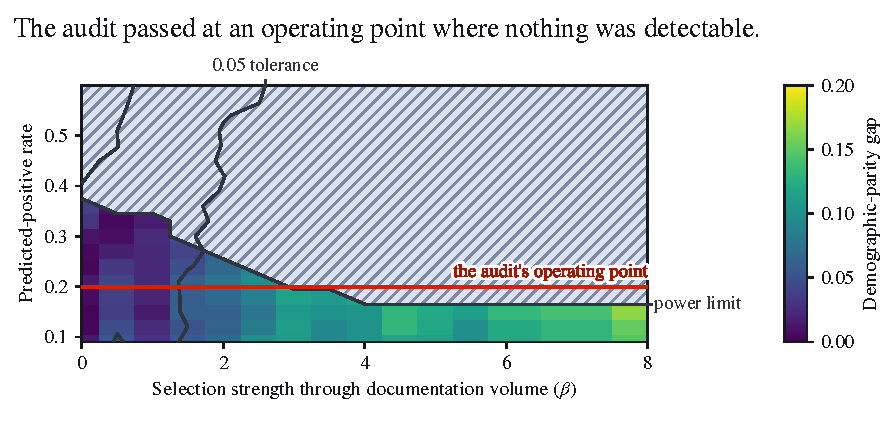
\includegraphics[width=0.98\linewidth]{figures/fig-threshold-surface.pdf}
\caption[Audited parity gap across operating points]{The audited
demographic-parity gap across operating points and selection strengths for
one selection experiment. The solid contour is the tolerance the audit was
written against. The hatched region is where the minimum detectable gap
exceeds that tolerance.}
\label{fig:appE-threshold-surface}
\end{figure}

The behaviour does not survive a controlled sweep of the same construct. A
simulator sweep over baselines, channel strengths and replicates inverts the
mapping between channel and drift direction; the grid's dimensions are not
registered, so none is quoted here. The direction in which a pool audit
drifts is therefore not a stable function of the selection channel that
produced the pool, at least across the region examined.

Five mechanism claims were proposed during this project to account for this.
Each was written down, each was tested against a parameter sweep, and each
failed; the record of those attempts is kept with the thesis's own
correction record, bound as an appendix to the thesis itself rather than
here. A sixth is not offered, and that restraint is a position rather than
an omission. The cheapest move available here is to build a story fitting
the two regimes actually observed. It would be unfalsified, because it would
be assembled after the fact from the data it purports to explain, and in the
write-up it would be indistinguishable from the five that already failed.

The supported claim is narrow and complete: on one population, with
baseline disparity fixed, the sign of the drift in a pool-level parity audit
is channel-dependent in a way a controlled sweep does not reproduce. Anyone
reading a single audited drift as evidence about an upstream selection
process is reading something whose direction was not stable where it was
checked. No subgroup harm is demonstrated, none is demonstrated anywhere in
this work, and these populations are simulated. No boundary for the effect
is claimed either, because the sweep that inverts the mapping is one
simulator with one functional form.


\end{document}
